\chapter{Modèles d'analyse de frontière stochastique pour l'optimisation des plans en curiethérapie HDD} \label{chapitre2} %  numéroté
\lettrine[nindent=0em,lines=2]{L}{}a Garantie de la qualité d’un traitement en curiethérapie nécessite la mise en place d’un programme de contrôle et de maintenance à plusieurs étages du processus de traitement. Rappelons de façon succincte que la qualité d’un traitement se mesure par l’habilité à traduire correctement les objectifs du traitement défini par le radio-oncologue en dose prescrite au volume cible tout en assurant la protection des OARs alentour. Sans être exhaustif, les grandes étapes permettant d’assurer et de maintenir la qualité des traitements consistent en: (1) la vérification des caractéristiques physiques des sources, (2) la vérification du fonctionnement des projecteurs de source ainsi que, (3) la vérification des systèmes de planification des traitements.
%
\begin{itemize}[label=\textbullet, font=\LARGE]
\item \textbf{Vérification des caractéristiques physiques}\newline
La vérification du certificat d’étalonnage des sources est une étape importante dans la démarche du maintien de la qualité. En effet, plusieurs études menées dans le but de comparer les caractéristiques physiques des sources fournies par les constructeurs à celles réellement mesurées ont permis de déceler des variations non négligeables; ces variations sont à l’origine des recommandations sur la vérification systématique du certificat de calibration des sources dès leur réception\cite{Baltas@1999, Elfrink@2002, Venselaar@1995}. Cette vérification peut porter, entre autres, sur la nature de la source proprement dite, le contrôle de conformité du certificat de calibration, l’homogénéité ainsi que la vérification de l’activité de chacune des sources avec une tolérance dans la variabilité de ± 10\% \cite{HaieMeder@2002}. La plupart des centres, en occurrence l’HDQ, utilisent les valeurs mesurées au sein de leurs services comme valeurs de référence dans le système de dosimétrie.
\\
%
\item \textbf{Vérification du fonctionnement des projecteurs de sources }\newline
Les projecteurs de sources jouent deux rôles fondamentaux dans le processus de planification, notamment, la radioprotection et de la dosimétrie. En curiethérapie HDD, ils sont responsables d’exécuter la programmation de la position de la source dans les différents cathéters implantés dans le CTV. Les tests recommandés pour assurer le bon fonctionnement d’un projecteur de source sont divers, parmi lesquels, la vérification de la précision de la position de la source au sein des cathéters d’une part \enquote{dwell position}, et d’autre part, la vérification sur la sélection du canal approprié tel que programmé lors de la planification. Le groupe de travail de l’AAPM TG-56 \cite{Nath@1997} recommande une précision sur la position de la source de ± 2 mm relative au système de référence de l’applicateur, et une tolérance de ± 2\% dans la vérification des temps d’irradiation à chacune des positions \enquote{dwell time}.
%
\item \textbf{Vérification des systèmes de planification des traitements}\newline
La vérification indépendante du calcul optimisé de la dose par un TPS avec une technique manuelle de calcul permettant de détecter des erreurs significatives avant chaque traitement constitue toujours un défi pour les physiciens, compte tenu de la contrainte sur le délai qui sépare le processus de planification et la délivrance de la dose au patient. Plusieurs approches de vérification ont été proposées dans la littérature \cite{Thomadsen@1992, Kubo@1992, Saw@1998} dont une consiste à considérer un point assez éloigné de l’implant de telle sorte que l’effet cumulatif des sources dans l’implant soit assimilable à une source ponctuelle; l’approximation de l’inverse carré de la distance peut ainsi être appliquée pour le calcul manuel afin de comparer le résultat à la valeur prédite par le TPS. En 2006, Rupak et al.\cite{Rupak@2006} ont proposé une méthode de vérification basée sur les DVHs. Bien que la précision de l’algorithme d’optimisation implémenté dans le TPS ait été évaluée lors de la phase du commissionnement de ce dernier, ce calcul indépendant permet cependant de vérifier, entre autres que les caractéristiques physiques des sources qui ont servi au calcul de la dose sont correctement prises en compte au cours de la planification (nature de la source, activité, date de traitement, décroissance radioactive), et qu’un éventuel bug dans le TPS n'a pas affecté le calcul de la dose.
\end{itemize}
%
La présentation succincte ci-dessus ne couvre certainement pas tous les aspects du contrôle de la qualité des plans en curiethérapie HDD, mais donne une idée sur l’approche classique recommandée dans la littérature et unanimement adoptée par les centres de radio-oncologie pour garantir la qualité des traitements. Cette approche est cependant complètement différente de celle adoptée dans le présent travail, bien que celle-ci se focalise également sur l’aspect de l’amélioration de la qualité des plans. L’approche basée sur l’AFS sur laquelle s’appuie le présent projet est un nouveau concept que nous introduisons en physique et doit être perçue comme complément à l’approche classique brièvement présentée ci-dessus; les deux ayant pour objectif global de garantir le contrôle tumoral sans délivrer de doses inutiles aux OARs.
%
\section{Formalisme de frontière stochastique}
L’analyse de frontière stochastique (AFS) \nomenclature{AFS}{Analyse de Frontière Stochastique} est une méthode développée en économie pour évaluer les performances d’une entreprise. La méthode repose sur la modélisation du processus de production permettant de prédire la quantité maximale d’extrants qui peut être produite, sur la base d’un vecteur d’intrants pour une technologie donnée. Aigner et al.\cite {aigner@2004} et Meeusen et al.\cite {meeusen@2004} furent les premiers pionniers à s’investir dans ce processus de modélisation, en proposant indépendamment et simultanément, un modèle de frontière qui prend en considération à la fois les éléments considérés comme exogènes au processus de production d’une entreprise, et les éléments représentés par l’efficience technique. La représentation mathématique d’une telle approche est donnée par l’équation \eqref{eqn:Frontiere},
%
\begin{equation}\label{eqn:Frontiere}
	y_{i} = f(x_{i}; \beta) + \epsilon_{i},  \quad \epsilon_{i} = v_{i} \mp u_{i}
\end{equation}
%
dans laquelle $y_{i} $ est un vecteur d’extrants pour la firme $ i $, $x_ {i} $ un vecteur d’intrants et $\beta $, un vecteur de paramètres à déterminer au cours du processus d’optimisation. Le terme d’erreur $\epsilon_ {i} $ est décomposé en deux composantes, un terme $v_{i}$ purement aléatoire et symétrique modélisant tous les facteurs qui ne sont pas sous le contrôle de l’entreprise, mais qui peuvent influencer la productivité de celle-ci (température, prix des matières premières, fluctuation du cours des actions, ou tout simplement la chance). Les $v_{i} $ sont supposés être iid selon N$(0, \sigma^{2}_{v})$. Cette composante aléatoire peut avoir une influence positive ou négative dans la productivité de l’entreprise en la déplaçant respectivement au-dessus ou au-dessous de sa frontière. $u_{i}\geq 0$ est un terme d’efficience technique associé aux facteurs contrôlables par la firme (efficacité ou la compétence des employés). $u_{i}$ est supposé indépendant de $v_{i}$ et distribué selon une loi normale tronquée positive, $N^{+}(0, \sigma^{2}_{u})$. Si les facteurs contrôlables par la firme sont correctement gérés, celle-ci devrait atteindre sa productivité maximale donnée par la frontière [$f(x_{i}; \beta) + v_{i}$]. Les signes $\mp$ dans l’équation \eqref{eqn:Frontiere} correspondent respectivement à une frontière de production et à une frontière de coût. La frontière de production prédit le maximum d’extrants sur la base d’un ensemble d’intrants, alors que la frontière de coût est associée à la minimisation des coûts de la production, c’est-à-dire, elle détermine le maximum de dépense devant être associée à une productivité maximale donnée. La forme analytique de la fonction $f(x_{i}; \beta)$ la plus utilisée dans la littérature est la fonction de Cobb-Douglas \cite{cobb@2004} donnée par l’équation \eqref{eqn:Chp2Cobb}:
%
\begin{equation}\label{eqn:Chp2Cobb}
	y_{i} = c \times \prod_{i} x^{\propto_{i}}_{i}
\end{equation}
%
dans laquelle $c > 0$  et $\alpha_{i} \in \Re$. La figure \ref{FrontiereCTV} ci-dessous illustre un exemple d’une frontière de production. La région mise en évidence en jaune identifie les firmes qui sont économiquement efficientes (productivité maximale atteinte pour un même vecteur d’intrants).
%
\begin{figure}[ht!]
\centering
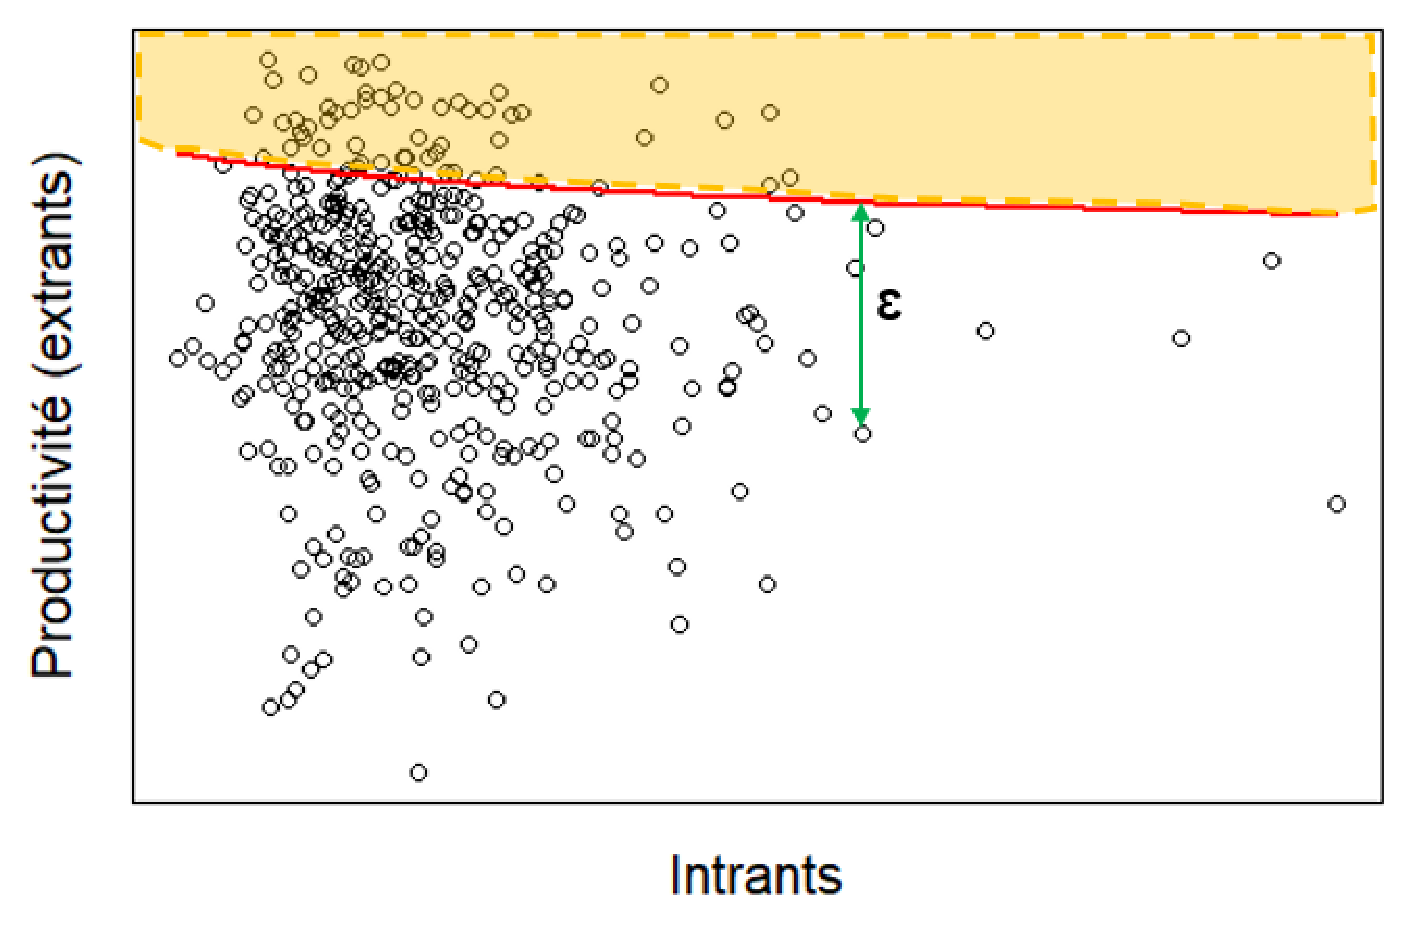
\includegraphics[width=8.5cm,height=5.8cm]{FrontiereCTV}
\caption{\label{FrontiereCTV} Illustration graphique de la frontière de production. $\epsilon$ est la distance entre la production d'une entreprise donnée par rapport à sa valeur prédite par la frontière.}
\end{figure}
%
La densité de probabilité conjointe, $f(u, v)$, sous l'hypothèse de l'indépendance des deux distributions $(u, v)$ est donnée par la relation:
%
\begin{equation}\label{eqn:fs1a}
f(u, v)=\frac{1}{\pi\sigma_{u}\sigma_{v}}exp\left[-\left(u^{2}/2\sigma^{2}_{u}\right)-\left(v^{2}/\sigma^{2}_{v}\right)\right]
\end{equation}
%
Dans le cas d'une frontière de production, en remplaçant $v$ par $u-\epsilon$ dans l'équation \ref{eqn:fs1a} et en intégrant dans le domaine de variabilité de $u$, c'est-à-dire, $[0, +\infty[$, on obtient la densité de probabilité de $\epsilon$ donnée par l'équation (\ref{eqn:fs2a}),
%
\begin{equation}\label{eqn:fs2a}
f\left(\epsilon_{i}\right) = \frac{2}{\sigma\sqrt{2\pi}}\left[1-\Phi\left(\frac{-\epsilon_{i}\lambda}{\sigma}\right)\right]exp\left(\frac{-\epsilon^{2}_{i}}{2\sigma^{2}}\right)
\end{equation}
%
dans laquelle, $\sigma = \sqrt{\sigma^{2}_{u}+\sigma^{2}_{v}}$ représente la largeur de la distribution, $\lambda=\sigma_{u}/\sigma_{v}$ son asymétrie, ou une mesure de la variabilité relative des deux sources d’erreurs. $\Phi\left(.\right)$ est la fonction de répartition d’une loi normale centrée réduite. Les différentes valeurs de $\lambda$ déterminent la nature de la frontière. Lorsque $\lambda = 0$, seule la composante aléatoire gouverne la distribution donnée par l’équation (\ref{eqn:fs2a}) et la frontière devient un simple ajustement. Une valeur élevée de $\lambda$ ($\lambda \rightarrow +\infty$) signifie que les facteurs qui sont sous le contrôle de l’entreprise sont dominants dans le manque de la production maximale, la frontière prend alors un caractère déterministe et la distribution de l'équation (\ref{eqn:fs2a}) devient celle d’une loi normale tronquée négative. L’espérance mathématique et la variance de $\epsilon$ sont décrits respectivement par les équations (\ref{eqn:fs3a}) et (\ref{eqn:fs4a}),
%
\begin{equation}\label{eqn:fs3a}
E\left(\epsilon\right)=E\left(u\right)=-\sqrt{\frac{2}{\pi}}\sigma_{u}
\end{equation}
%
\begin{equation}\label{eqn:fs4a}
V\left(\epsilon\right)=V\left(u\right)+V\left(v\right)=\left(\frac{\pi-2}{\pi}\right)\sigma^{2}_{u}+\sigma^{2}_{v}
\end{equation}
%
Les équations similaires pour une frontière de coût peuvent être déduites des équations (\ref {eqn:fs1a}-\ref{eqn:fs4a}) en y remplaçant $\epsilon $ par $ -\epsilon $. La figure \ref {DensiteProb} ci-dessous illustre la forme de la densité de probabilité de la variable $\epsilon$ donnée par l'équation (\ref{eqn:fs2a}), respectivement pour une frontière de production (a) et une frontière de coût (b).
%
\begin{figure}[ht!]
  \centering
  \subfloat[Frontière de production]{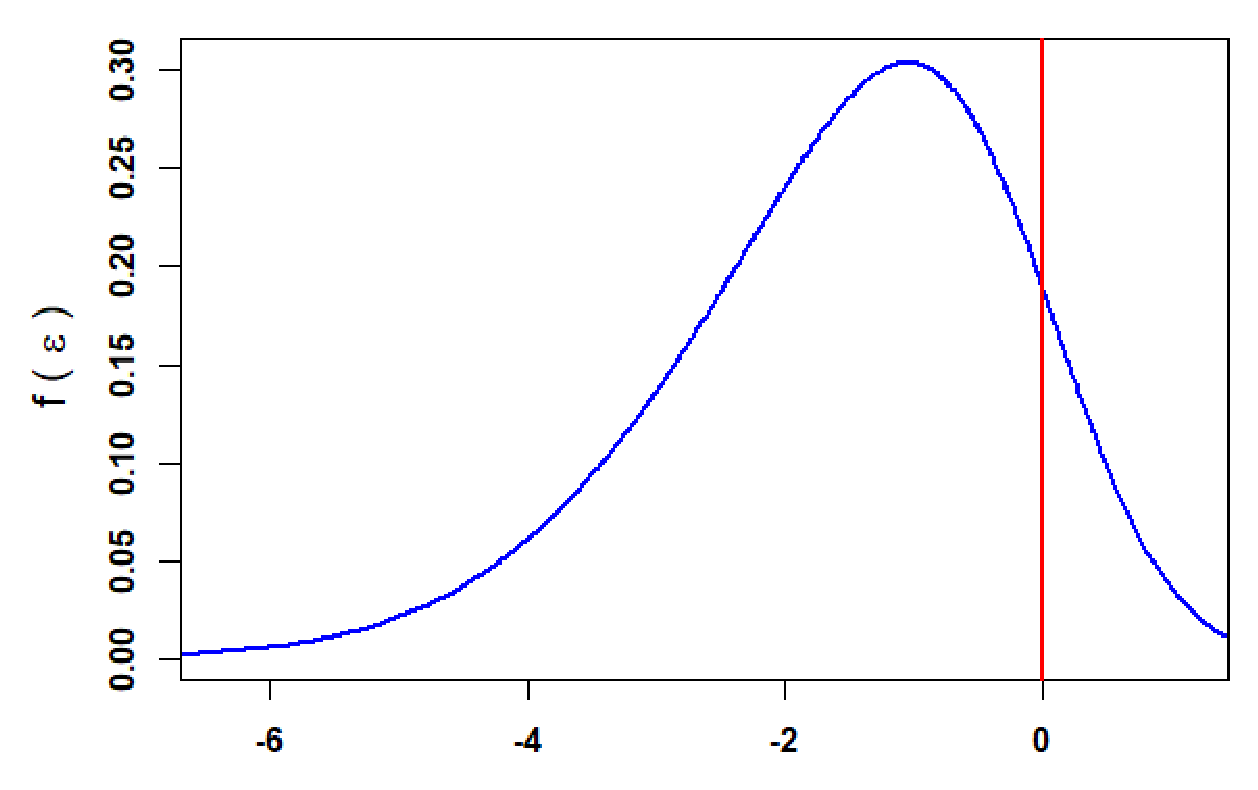
\includegraphics[width=7.1cm,height=5.2cm]{DensiteProbA}\label{fig:f1}}
  \hspace{0.5cm}
  \subfloat[Frontière de coût ]{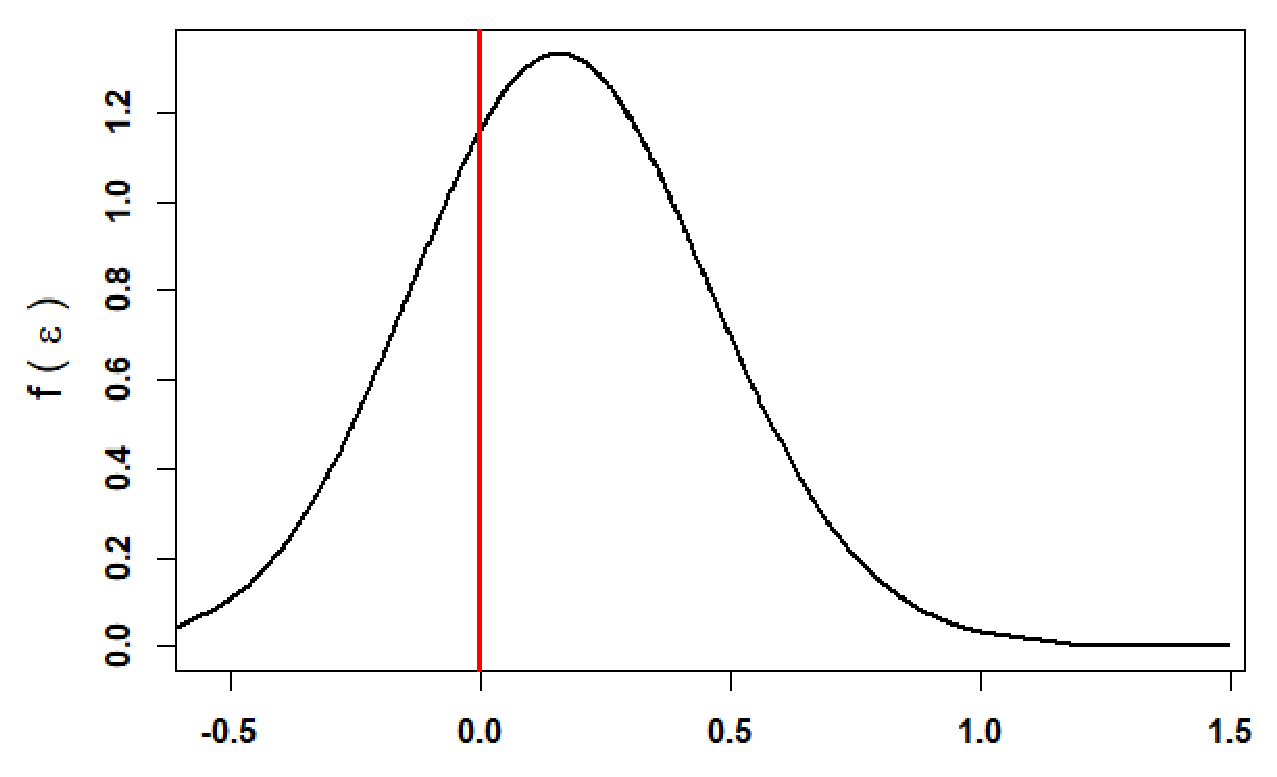
\includegraphics[width=7.2cm,height=5.2cm]{DensiteProbB}\label{fig:f2}}
\caption{\label{DensiteProb} Illustration d'une distribution tronquée négative (a) et tronquée positive (b). Les deux cas correspondent au scénario pour lequel la composante déterministe $u$ de $\epsilon$ est dominante.}
\end{figure}
%
L’utilisation de ce formalisme d'AFS dans le contexte de l’optimisation des plans en curiethérapie HDD repose dans le développement des modèles de frontière de production pour les paramètres dosimétriques que l’on cherche à maximiser au cours de la planification (couverture du CTV), et de frontières de coût pour ceux qui sont sujets à la minimisation (OARs). La forme analytique de la frontière présentée dans l’équation (\ref{eqn:Chp2Cobb}) a été modifiée dans son application. En effet les paramètres géométriques $x_{i}$ de cette équation ont été remplacés par un profil géométrique construit sous forme d’une combinaison linéaire desdits paramètres, suivant l’équation (\ref{eqn:Chp2Cobb2})
%
\begin{equation}\label{eqn:Chp2Cobb2}
	y_{i} = c\times \left(\sum_{i}\beta_{i}x_{i}\right)^{\alpha}
\end{equation}
%
Le passage de l’équation (\ref{eqn:Chp2Cobb}) à l’équation (\ref{eqn:Chp2Cobb2}) qui s’est fait sans perte d’informations contenues dans les modèles ($\sigma_{u}, \sigma_{v}$), présente l’avantage de visualiser les frontières dans un graphique à deux dimensions lorsque le nombre de paramètres géométriques impliqué dans le processus de modélisation est supérieur à deux.
%
\section{Application à l'optimisation des plans en curiethérapie de la prostate HDD}
\subsection{Acquisition des échantillons}
La première phase de la modélisation a consisté en l’acquisition de deux échantillons indépendants. Un premier échantillon de 495 patients qui a servi dans la construction des modèles, correspond aux patients traités dans la plage mars 2013 - juillet 2016, et un deuxième échantillon de 100 patients traités en 2011 qui a servi de test. Les deux échantillons sont des patients traités en curiethérapie de la prostate HDD, en une fraction de 15 Gy, en complément après une radiothérapie externe. L'optimisation de la dosimétrie de ces patients s'est faite avec l'algorithme IPSA implémenté dans le TPS Oncentra Brachy (Elekta - Brachy, Veenendaal, The Netherlands).
%
\subsection{Description et extraction des paramètres géométriques} \label{Parag}
\subsubsection{Volume des structures (CTV, OARs)}
L’extraction des volumes des différentes structures (CTV, vessie, rectum et urètre) a été faite manuellement à partir du TPS pour les 100 premiers patients du premier échantillon. Le programme 3D Slicer a été utilisé pour faciliter l’extraction de ces volumes pour le reste des plans (premier et deuxième échantillon). L’extraction des paramètres géométriques s’est effectuée en deux étapes. Dans la première étape, les DVH des différents plans ont été extraits manuellement à partir de 3D Slicer et un script sous Python a permis l’automatisation de l’extraction des paramètres géométriques sur lesdits DVH. Le niveau de précision des volumes ainsi calculés a d’abord été évalué en comparant les valeurs calculées avec ceux extraits manuellement du TPS pour les 100 premiers patients. Pour le CTV, la vessie et le rectum, les écarts relatifs moyens des différents volumes calculés, entre le TPS et 3D Slicer sont respectivement de de 2,02\% ($\sigma = 0,578 $), 1,14\% ($\sigma = 0,544 $) et 1,90\% ($\sigma = 1,11 $). Pour le volume de l’urètre, l’écart absolu moyen entre 3D Slicer et le TPS est de 0,14 ($\sigma = 0,024 $). L’application des différents modèles de régression présentés dans la figure \ref{ModeleRegres} pour le calcul des volumes du CTV, du volume de la vessie et du volume du rectum a amélioré la précision des calculs, c’est-à-dire, la moyenne des écarts relatifs est passée des valeurs citées précédemment à 0,35\% ($\sigma = 0,24 $), 0,45\% ($\sigma = 0,55 $) et 0,93\% ($\sigma = 1,42 $), respectivement. L’écart absolu moyen pour le volume de l’urètre après correction est de 0,014 ($\sigma = 0,01 $). Ces modèles de régression ont été appliqués pour corriger toutes les valeurs des paramètres géométriques extraits des DVHs pour le reste des plans des deux échantillons.
%
\begin{figure}%[ht!]
  \centering
  \subfloat{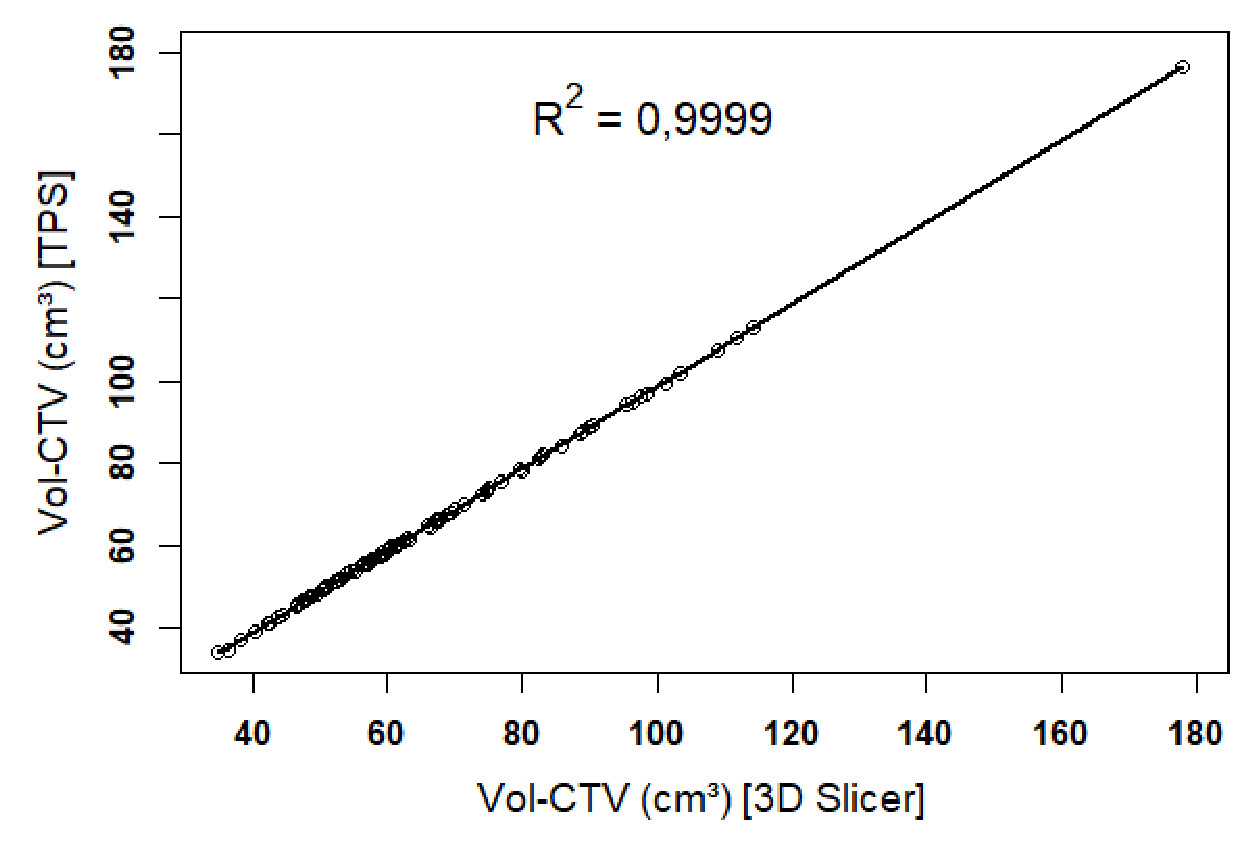
\includegraphics[width=7.2cm,height=5.2cm]{RegresCTV}\label{fig:RegresCTV}}
  \hspace{0.5cm}
  \subfloat{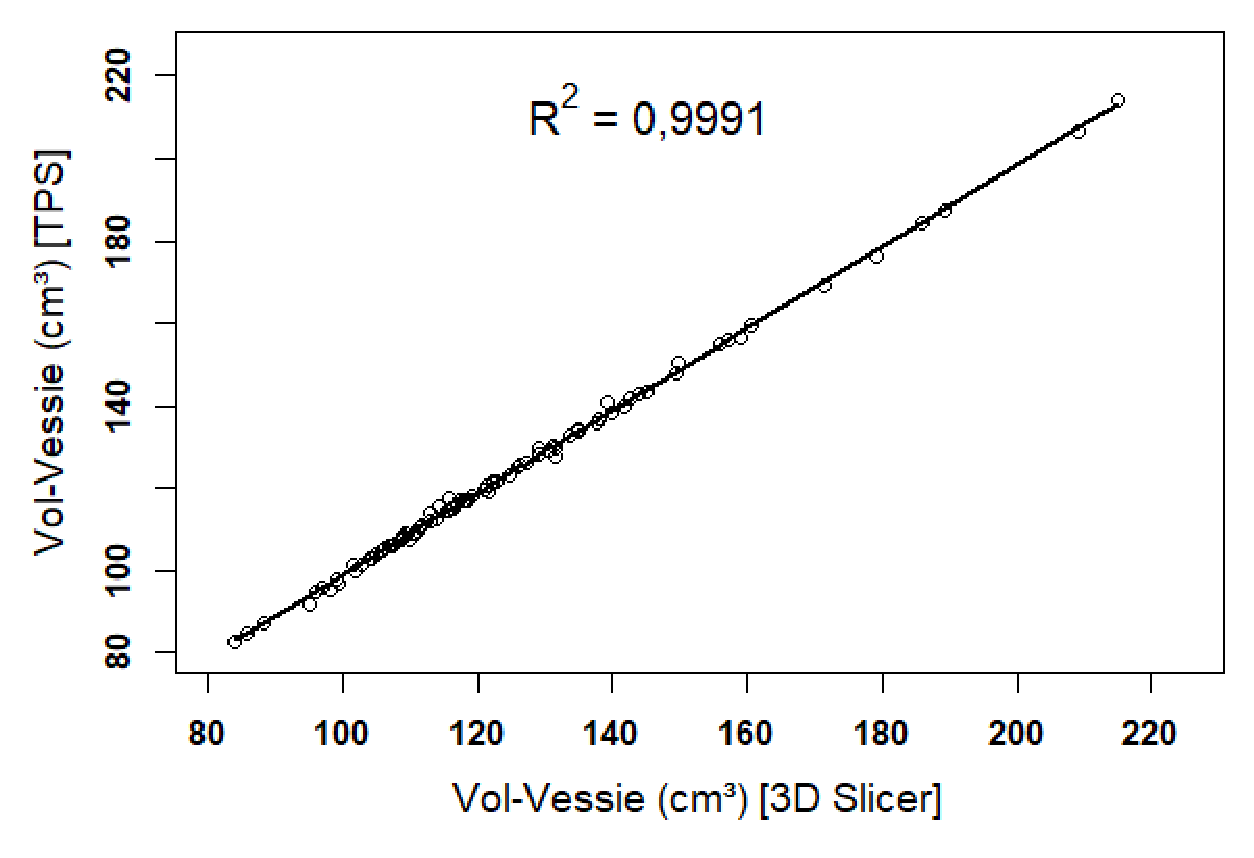
\includegraphics[width=7.2cm,height=5.2cm]{RegresVessie}\label{fig:RegresVessie}}
  \hspace{0.5cm}
  \subfloat{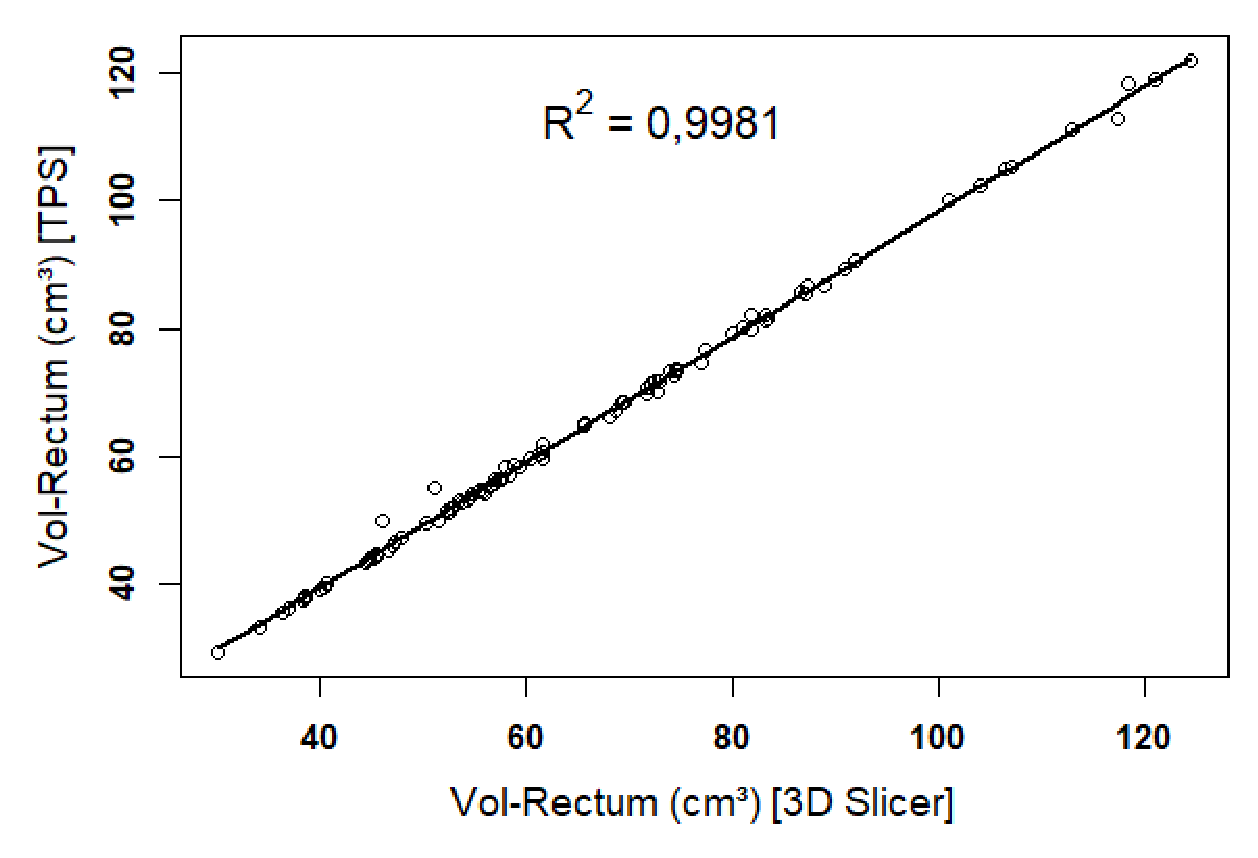
\includegraphics[width=7.2cm,height=5.2cm]{RegresRectum}\label{fig:RegresRectum}}
  \hspace{0.5cm}
  \subfloat{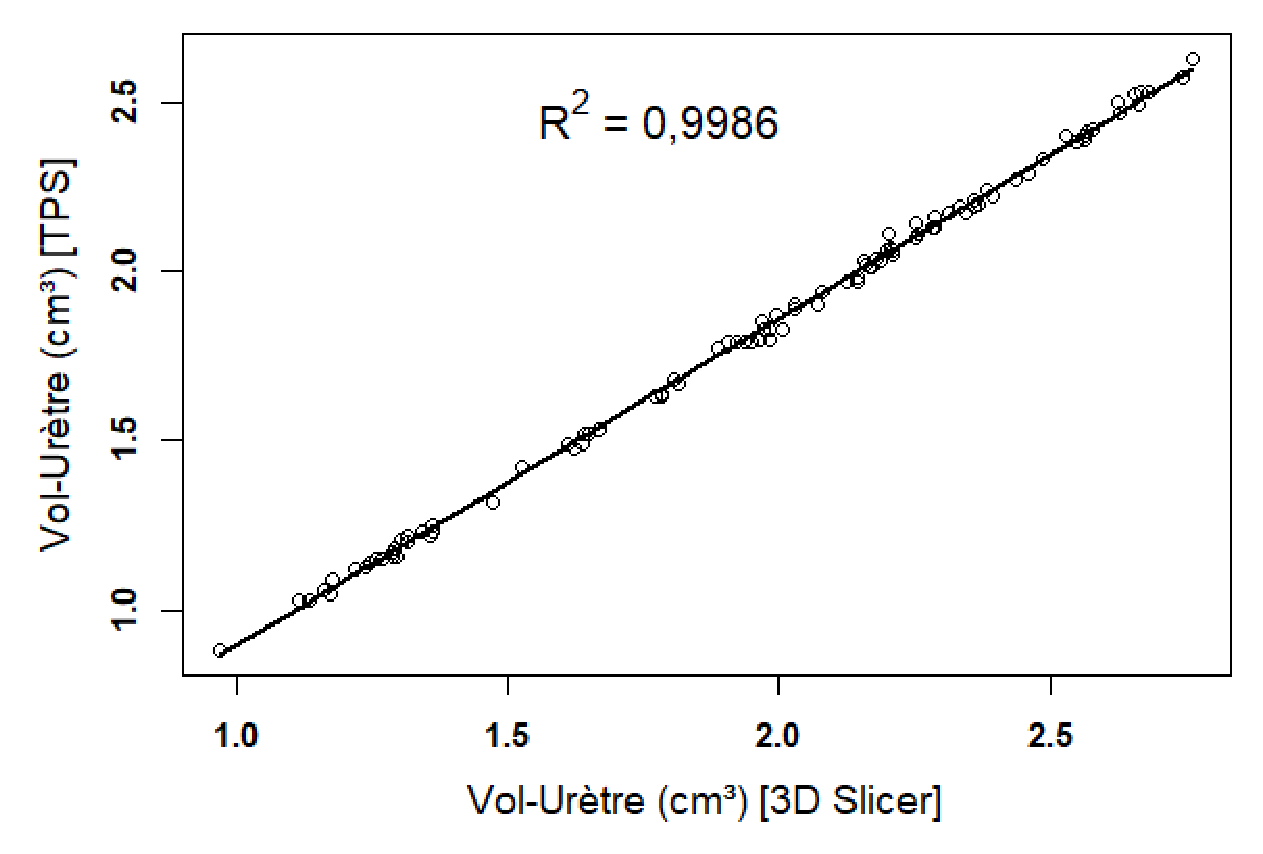
\includegraphics[width=7.25cm,height=5.2cm]{RegresUretre}    \label{fig:RegresUretre}}
  %\hspace{0.5cm}
\caption{\label{ModeleRegres} Résultats des modèles de régressions linéaires construits à partir des volumes calculés par 3D Slicer.}
\end{figure}
%
\subsubsection{Distance de Hausdorff CTV-OARs}
En mathématiques, et plus précisément en topologie, la distance de Hausdorff est un outil qui mesure l’éloignement de deux sous-ensembles d’un espace métrique sous-jacent. Celle-ci porte le nom de son inventeur, le mathématicien allemand Felix Hausdorff. Cette distance est tributaire de plusieurs propriétés qui lui confèrent son utilisation, entre autres, dans la reconnaissance des formes, la quantification des dissemblances entre deux formes géométriques, ou dans la numérisation des images. Elle a été utilisée dans le contexte du présent projet pour quantifier la distance entre le CTV et chaque OAR (vessie, rectum et urètre). Elle présente l’avance par rapport à la distance euclidienne, de quantifier la proximité relative entre deux structures tout en tenant compte de leurs formes respectives. Du point de vue formel, si on considère deux ensembles A et B bornés et non vides, la distance de Hausdorff entre les deux ensembles est le maximum de la fonction définie par l’équation (\ref{eqn:Hausdorff1}),
%
\begin{equation}\label{eqn:Hausdorff1}
	h (A, B) = max_{a\in A}\left\{min_{b\in B}\left\{d (A, B)\right\}\right\}
\end{equation}
%
dans laquelle, d (A, B) est n’importe quelle métrique entre A et B en général et en particulier, une distance euclidienne entre les deux ensembles dans le présent projet. Il convient cependant de souligner que la distance de Hausdorff est une distance orientée, c’est-à-dire, dans la plupart des cas, h (A, B) $\neq$ h (B, A), d’où la formulation plus générale donnée dans l’équation (\ref{eqn:Hausdorff2}),
%
\begin{equation}\label{eqn:Hausdorff2}
	H (A, B) = max\left\{h (A, B), h (A, B)\right\}
\end{equation}
%
\subsubsection{Divergence moyenne des cathéters}
Sous guidage échographique, les cathéters implantés dans le volume cible présentent généralement une certaine divergence entre elles; cette divergence, volontaire ou non, influence la dosimétrie. Ce paramètre a été évalué en deux étapes. Premièrement, les données permettant de reconstruire les cathéters ont été extraites des fichiers DICOM et les cathéters ont été reconstruits (figure \ref{Catheters}A), puis découpés aux dimensions de la prostate (figure \ref{eqn:Hausdorff2}B). Les points rouges représentent les positions activées au sein de chaque cathéter. Deuxièmement, la divergence moyenne des cathéters a été évaluée en calculant la pente moyenne; celle-ci a été échantillonnée dans chaque cathéter sur tous les deux (respectivement, trois points), si le nombre de points permettant de reconstruire ledit cathéter est pair (respectivement, impair). Une divergence moyenne globale a été ensuite déduite en moyennant la pente dans l'ensemble des cathéters.
%
\begin{figure}[ht!]
\centering
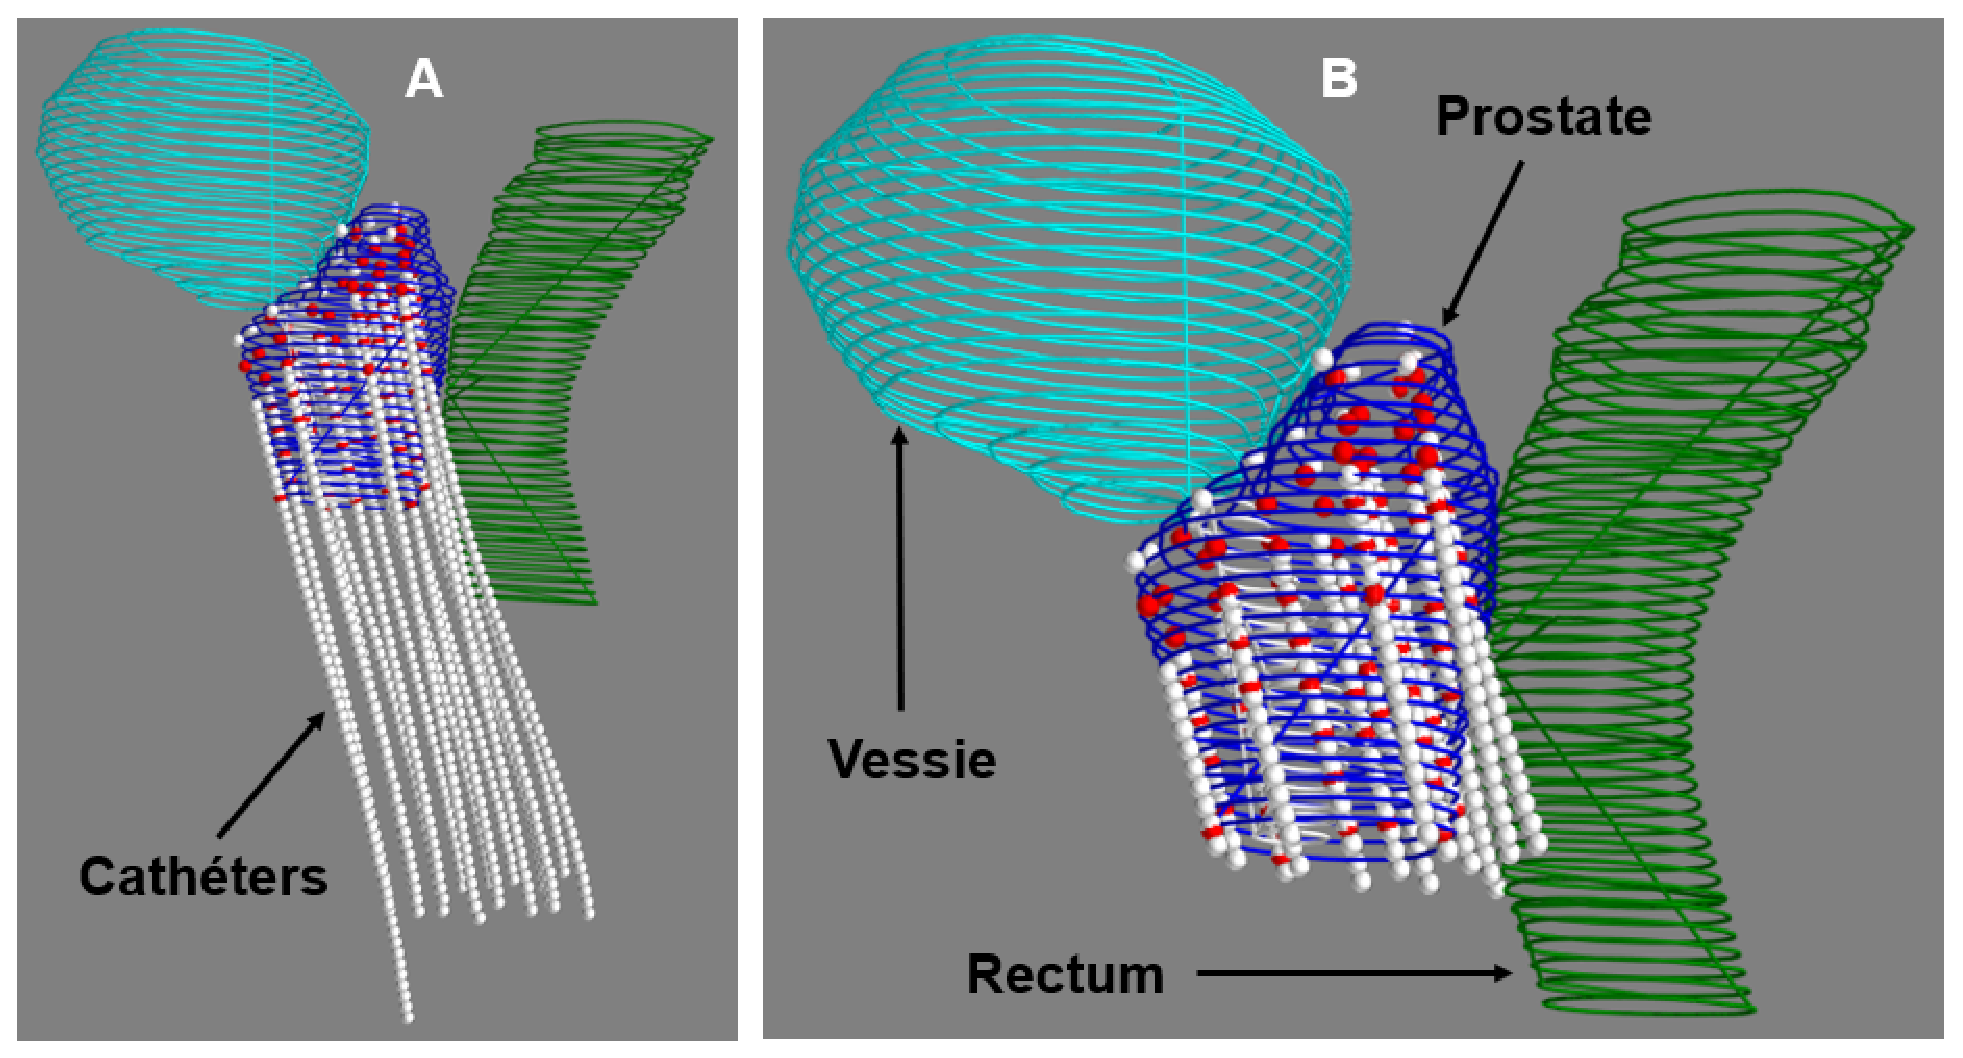
\includegraphics[width=10.5cm,height=5.8cm]{Catheters}
\caption{\label{Catheters} Illustration du processus d'évaluation de la divergence des cathéters dans le volume cible.}
\end{figure}
%
\subsection{Paramètres dosimétriques d'intérêt}
Les paramètres dosimétriques impliqués dans le processus de modélisation sont ceux qui guident le processus d'optimisation au cours de la planification, et qui sont recommandés soit par le RTOG 0924 \cite{RTOG} ou l'ABS \cite{ABS} et qui présentent une certaine variabilité inter-patients. Ces paramètres sont résumés dans le tableau \ref{IndicesDosim} ci-dessous.
%
\begin {table*}[!ht]
\captionsetup{singlelinecheck=off, skip=4pt, width =\dimexpr \textwidth-2cm\relax}%
\caption{Paramètres dosimétriques sur lesquels les modèles sont construits.}
\label{IndicesDosim} 
\renewcommand{\arraystretch}{1.4}
\vspace{-0.2cm}
\begin{center}
\begin{tabular}{llrrrrrrrrrrrr}
\toprule[1.3pt]
\hline
\multicolumn{1}{l} \textbf{Structures d'intérêts} & {} & {} & {} & {} & \multicolumn{5}{c} \textbf{Indices dosimétriques} & {} & {} \\
\cline{3-13}
\multicolumn{1}{c}{\scriptsize \textbf{}} & {} & V$_{130}$ & {} &  V$_{125}$ & {} &  V$_{100}$ & {} &  V$_{75}$ & {} &  D$_{10}$ & {} & {} \\
\hline
 \textbf{CTV} & {} & {} & {} & {} & {} & x & {} & {} & {} & {} & {} \\
\vspace{0.1cm}
%
\textbf{Vessie} & {} &  {} & {} & {} & {} &  {} & {} & x & {} & {} & {} \\
% 
\textbf{Rectum} & {} &  {} & {} & {} & {} &  {} & {} & x & {} & {} & {} \\
%
\textbf{Urètre} & {} &  x & {} & x & {} & {} &  {} & {} & {} & x & {} \\
\bottomrule[1.3pt]
\end{tabular}
\end{center}
\end{table*}
%
Pour les indices dosimétriques présentés dans le tableau ci-dessus, V$_{x}$ désigne le pourcentage du volume recevant au moins $x$\% de la dose prescrite, tandis que D$_{x}$ est la dose reçue par un pourcentage $x$ du volume irradié. L'ABS recommande une couverture minimale du CTV de 90\%, tout en minimisant la dose aux OARs (V$_{75}$ pour la vessie et le rectum < 1 cm$^{3}$) et V$_{125}$ pour l'urètre < 1 cm$^{3}$. Un réajustement de l’implant est recommandé par cet organisme si les limites de doses aux OARs pour un plan donné ne peuvent pas être obtenues. D'autre part, V$_{130}$ (respectivement D$_{10}$) qui sont des paramètres recommandés par le RTOG 0924 devraient être maintenus en dessous de 118\% de la dose de prescription (respectivement égal à zéro). Les indices dosimétriques qui ont fait l'objet de la modélisation sont V$_{100}$, V$_{75}$ et D$_{10}$; V$_{130}$ et V$_{125}$ étant nulles pour l'échantillon considéré. L'approche dans l'automation de l'extraction de ces indices dosimétriques à partir de DVHs extraits de 3D Slicer a été la même que celle présentée dans la sous-section \ref{Parag}. La figure \ref{ModeleRegresIndice} illustre les modèles de régression obtenus pour les indices dosimétriques D$_{10}$ (normalisée à la dose de prescription) et V$_{75}$ pour le rectum.
%
\begin{figure}[ht!]
  \centering
  \subfloat{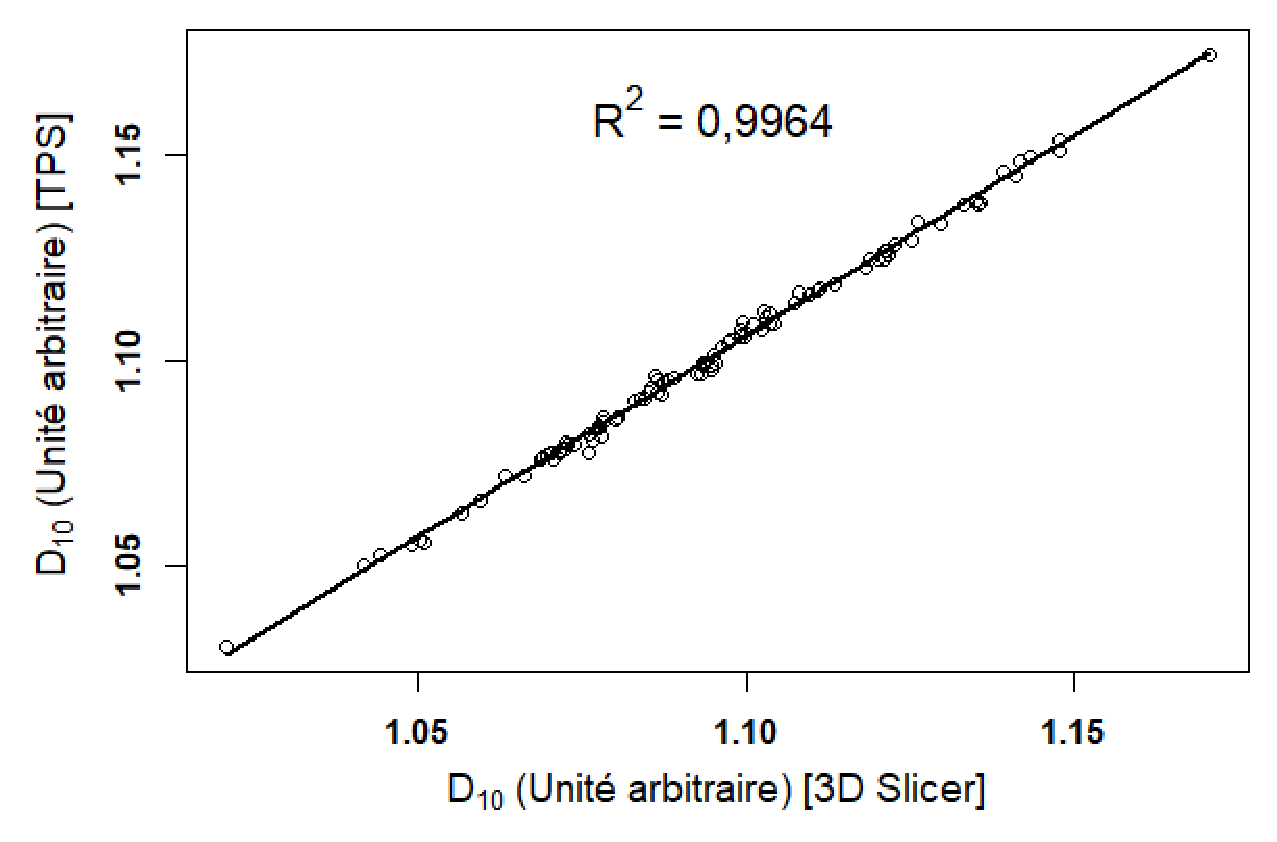
\includegraphics[width=7.2cm,height=5.2cm]{RegresD10U}\label{fig:RegresD10U}}
  \hspace{0.5cm}
  \subfloat{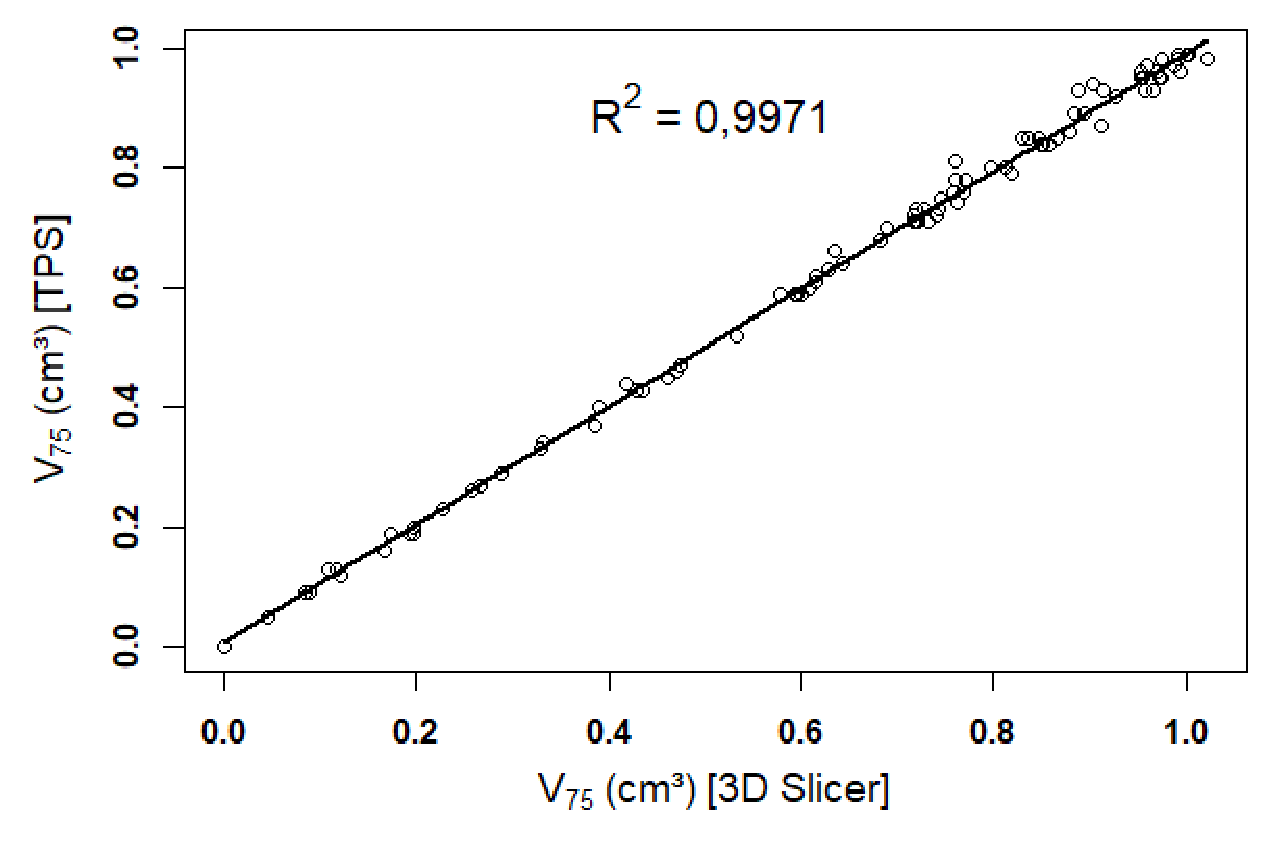
\includegraphics[width=7.2cm,height=5.2cm]{RegresV75R}\label{fig:RegresV75R}}
  \hspace{0.5cm}
\caption{\label{ModeleRegresIndice} Modèles de régression linéaire des indices dosimétriques construits à partir des DVHs extraits de 3D Slicer.}
\end{figure}
%
\section{Processus d'optimisation}
\subsection{Outil d'optimisation}
Les différentes frontières ont été optimisées avec la méthode de maximisation de la vraisemblance avec le logiciel statistique R \cite{R@2017}; le processus d'optimisation a donc consisté pour chaque modèle, à déterminer les valeurs des paramètres optimales de \enquote{c} et \enquote{$\beta$} de l'équation (\ref{eqn:Chp2Cobb2}) qui maximisent cette vraisemblance. Le logiciel R en lui-même est un logiciel de statistique gratuit et à code source ouvert (open-source). Il présente ce double avantage d'être à la fois un langage informatique (langage interprété) et un environnement de travail permettant de réaliser des analyses statistiques telles que: la statistique descriptive, les tests d’hypothèses les méthodes de régression linéaire (simple et multiple). Le logiciel R implémente plusieurs algorithmes d'optimisation, parmi lesquels, les algorithmes basés sur les gradients (Nelder-Mead ; quasi-Newton ; gradient conjugué ; BFGS quasi-Newton ; SANN) et un algorithme basé sur le recuit simulé GenSA \cite{GenSA@2012}. Les algorithmes basés sur les gradients qui sont implémentés dans la fonction \enquote{optim} dans R présentent un inconvénient majeur, leur difficulté à ne pas être piégés dans les minima locaux. D'autre part, la fonction \enquote{optim} n'offre pas la possibilité d'imposer des contraintes sur les paramètres à optimiser, exemple de $\sigma_{u} ≥ 0$ et $\sigma_{v} ≥ 0$. L’algorithme GenSA, du fait qu'il soit basé sur le recuit simulé, permet de traiter les problèmes plus complexes (fortement non linéaire); il est donc capable de sauter plusieurs minima locaux qui ne sont pas réellement optimaux. Il est également plus flexible du fait qu'il offre la possibilité de définir le domaine de variabilité des différents paramètres à optimiser tout en les imposant des contraintes.
%
\subsection{Principe d'optimisation par la méthode de maximisation de la vraisemblance}
La méthode du maximum de vraisemblance développée en 1922 \cite{Stigler@2007, Aldrich@1997} par le statisticien Ronald Aylmer Fisher est une méthode statistique qui, à partir d’un échantillon observé, permet d’inférer les meilleures valeurs des paramètres d'une distribution de probabilité. Le principe de la méthode repose dans la construction d’une fonction dite de vraisemblance que l’on cherche à maximiser par rapport aux paramètres de la distribution inconnus. Soient $x_{1}$, $x_{2}$, $x_{3}$,…, $x_{n}$, $n$ observations indépendantes d’un phénomène continu \enquote{X} gouverné par une densité de probabilité $f_{\theta}$, la fonction de vraisemblance  $L(\theta)$ est donnée par l’équation (\ref{eqn:Vraisemb}),
%
\begin{equation}\label{eqn:Vraisemb}
	L (\theta) =\prod^{n}_{i=1}f\left(x_{i}, \theta\right)
\end{equation}
%
où $\theta$ est un vecteur de paramètres inconnus à déterminer au cours du processus d’optimisation. Dans la pratique, l'équation (\ref{eqn:Vraisemb}) est linéarisée pour faciliter la recherche de la solution, ce qui conduit à l'équation (\ref{eqn:Vraisemb2}),
%
\begin{equation}\label{eqn:Vraisemb2}
\mathcal{L} = \sum^{n}_{i=1}ln\left[f\left(x_{i}, \theta\right)\right]
\end{equation}
%
L'application de ce formalisme dans la recherche des paramètres optimaux d'un modèle de FS conduit à l'équation (\ref{eqn:Vraisemb3}) dans laquelle $\varphi (.)$ (respectivement $\Phi (.)$) sont la densité de probabilité d'une loi normale centrée et réduite (respectivement sa fonction de partition).
%
\begin{equation}\label{eqn:Vraisemb3}
\mathcal{L} = \sum^{n}_{i=1}ln\left(\frac{2}{\sigma}.\varphi\left(\frac{\epsilon_{i}}{\sigma}; 0; 1\right).\left[1-\Phi\left(-\epsilon_{i}\frac{\lambda}{\sigma};0;1\right)\right]\right)
\end{equation}
%
Les contraintes imposées aux paramètres des équations (\ref{eqn:Chp2Cobb2}) et (\ref{eqn:Vraisemb3}) sont telles que $\sigma_{u} ≥ 0$ et $\sigma_{v} ≥ 0$; $c$, $\beta$ et $\alpha$ des réels. Il convient cependant de souligner qu'une valeur négative du paramètre \enquote{c} n'a pas de sens physique, toutes les observations étant positives, mais le fait d'élargir le domaine de variabilité de ce paramètre dans l'ensemble des nombres réels donne assez de marge de manœuvre à l'algorithme GenSA dans la recherche des paramètres optimaux.
%
\section{Résultats des optimisations}
\subsection{Corrélation linéaire entre les paramètres géométriques et dosimétriques}
La phase de la modélisation des FS a été précédée par une recherche de corrélation linéaire simple entre chaque indice dosimétrique d'intérêt et chaque paramètre géométrique, bien qu'une telle corrélation ne soit pas nécessaire pour que ce paramètre puisse contribuer à la construction du modèle de FS associé avec une importance statistiquement significative. En effet, les modèles de FS ne correspondent pas à des ajustements, mais plutôt en la comparaison des plans de l'échantillon, chacun ayant un profil de paramètres géométrique qui lui est propre. L'ensemble des résultats montre qu'aucune corrélation linéaire claire ne peut être dégagée entre chacun des paramètres géométriques et les différents indices dosimétriques. La figure \ref{ModeleRegresPG} illustre un exemple de la qualité de la régression entre la couverture du CTV et son volume ou entre la couverture du CTV et le volume du rectum. 
%
\begin{figure}[htt!]
  \centering
  \subfloat{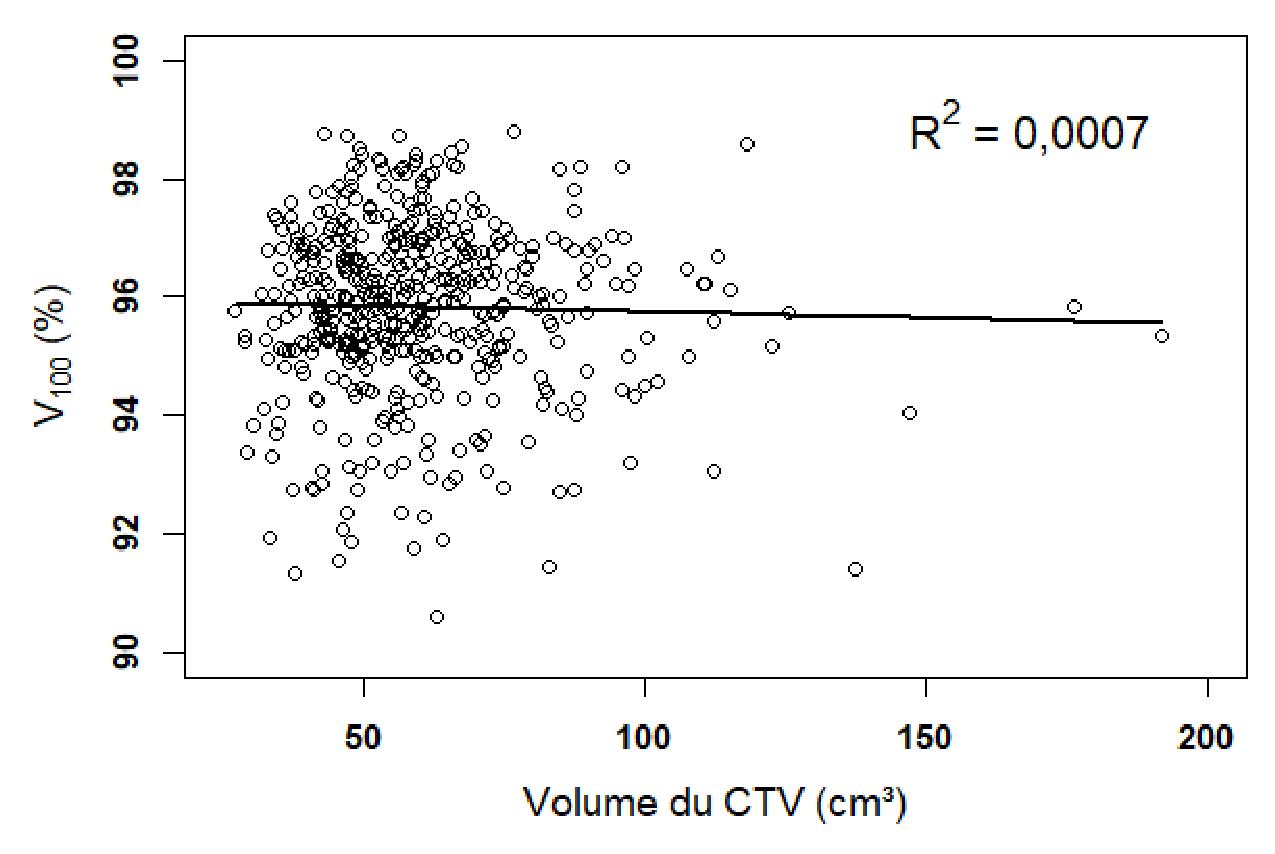
\includegraphics[width=7.2cm,height=5.2cm]{RegresV100-VolCTV}\label{fig:RegresV100-VolCTV}}
  \hspace{0.5cm}
  \subfloat{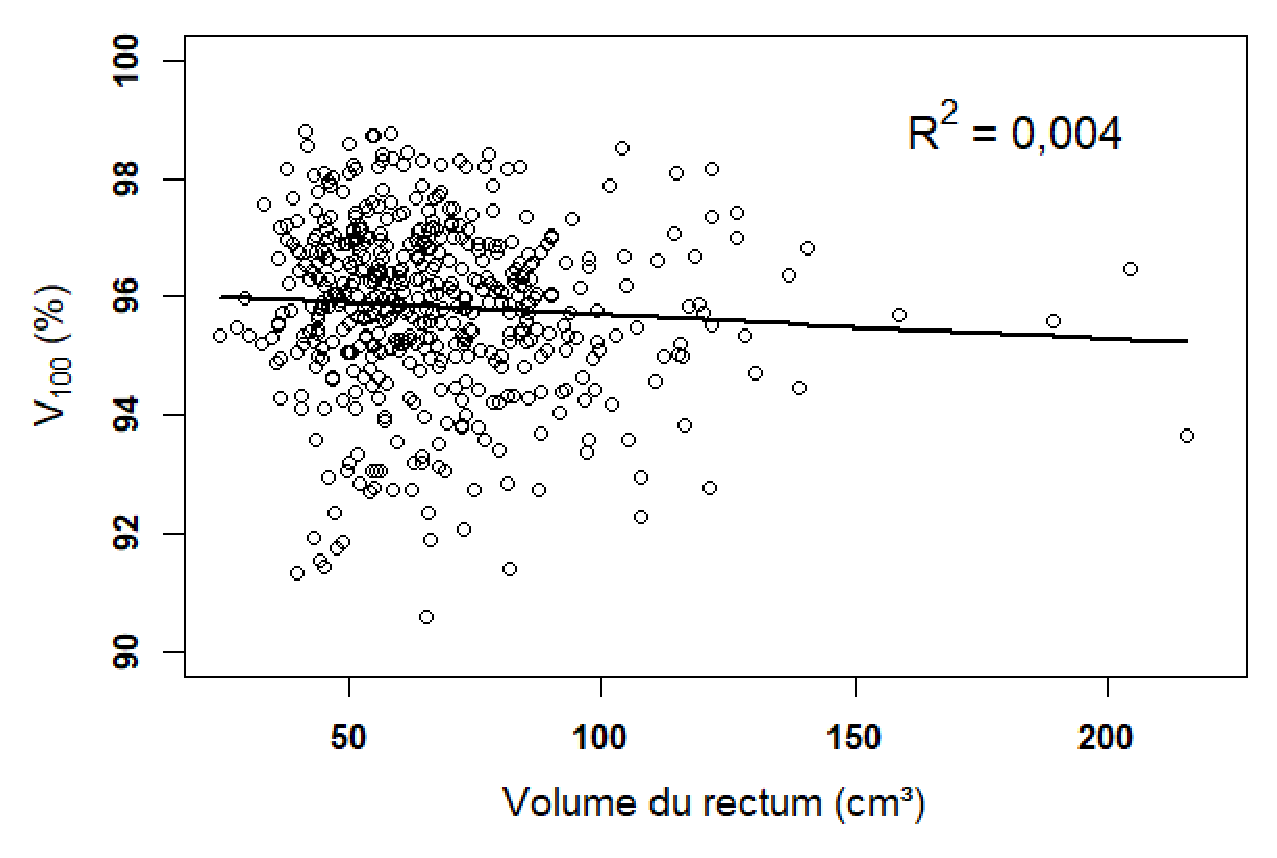
\includegraphics[width=7.2cm,height=5.2cm]{RegresV100-VolRectum}\label{fig:RegresV100-VolRectum}}
  \hspace{0.5cm}
\caption{\label{ModeleRegresPG} Modèles de régression linéaire pour la couverture du CTV en fonction du volume du CTV et le volume du rectum.}
\end{figure}
%
Le tableau \ref{coeffDeterm} résument les valeurs du coefficient détermination obtenues pour les différents modèles de régression et pour l'ensemble des paramètres géométriques.
%
\begin {table}[ht!]
\caption{Résumé de la qualité de la régression linaire simple entre chaque paramètre dosimétrique d'intérêt et les différents paramètres géométriques. Les lettres R, V et U désignent le rectum, la vessie et l'urètre, respectivement. Vol-x et Haus-x font référence, respectivement, au volume de l'organe x et à la distance de Hausdorff entre le CTV et l'organe x. P-moy est la pente moyenne des cathéters dans le CTV.}
\label{coeffDeterm} 
\renewcommand{\arraystretch}{1.4}
\begin{tabular}{llrrrrrrrrrrr}
\toprule[1.3pt]
\hline
\multicolumn{1}{l} \textbf{Modèles} & {} & {} & \multicolumn{5}{c} \textbf{Coefficient de détermination (R$^{2}$)} \\
\cline{3-10}
\multicolumn{1}{c}{\scriptsize \textbf{}} & {} & Vol-CTV & Vol-R &  Vol-V &  Vol-U & P-moy & Haus-R & Haus-V & Haus-U \\
\hline
 \textbf{V$_{100}$} & {} & 0,0007 & 0,0042 & 0,0099 & 0,0343 & 0,0012 & 0,0113 & 0,0167 & 0,0001  \\
\vspace{0.1cm}
%
\textbf{V$_{75}$ (R)} & {} & 0,0962 &  0,0063 & 0,0019 & 0,0012 & 0,0166 &  0,0 & 0,0274 & 0,0790 \\
% 
\textbf{V$_{75}$ (V)} & {} & 0,0074 &  0,0147 & 0,0060 & 0,0049 & 0,0025 & 0,0018 & 0,0207 & 0,0083  \\
%
\textbf{D$_{10}$ (U)} & {} & 0,0033 &  0,0088 & 0.0 & 0,0055 & 0,0027 & 0,0052 &  0,0141 & 0,0047 \\
\bottomrule[1.3pt]
\end{tabular}
\end{table}
%
\subsection{Modèle de FS par paramètre géométriques}
La figure \ref{ModeleFS-VolCTV} présente le résultat des modèles de FS, qualifiés de modèles de base du fait qu'ils sont optimisés avec un seul paramètre géométrique, le volume du CTV. Les plans optimaux sont ceux situés au-dessus de la frontière pour le modèle V$_{100}$ (frontière de production), et en dessous des frontières pour les autres paramètres (frontières de coût). Le modèle correspondant au paramètre V$_{75}$ pour le rectum correspond à un ajustement ($\sigma_{u} = 0$). L’interprétation de ce résultat est que l’indice dosimétrique V$_{75}$ pour le rectum est un paramètre bien optimisé en clinique, son amélioration n’est donc plus possible pour l’ensemble des plans qui constituent l’échantillon. Par contre, on observe pour les autres paramètres pour le CTV, la vessie et l’urètre, qu’un grand nombre de plans sont localisés en dessous de la frontière pour V$_{100}$, et au-dessus de la frontière pour D$_{10}$  et V$_{75}$ (vessie); ceci témoigne que ces deux paramètres dosimétriques sont améliorables pour l’échantillon considéré et peuvent être prédits pour un nouveau plan caractérisé par le volume du CTV. La figure \ref{ModeleFS-Boxplot} résume la distribution de $\epsilon$ pour V$_{100}$ et V$_{75}$ (vessie) par paramètre géométrique; les résultats sont similaires dans le cas de D$_{10}$. Les plans optimaux sont ceux pour lesquels la variable aléatoire $\epsilon$, c'est-à-dire, l'écart entre le plan optimisé par le TPS Oncentra Brachy et celui prédit par la frontière est négatif pour le CTV et positif pour la vessie et l'urètre. Cependant, ces modèles ayant comme seul paramètre géométrique, le volume du CTV, ne sont pas représentatifs de la réalité, étant donné que la couverture de la prostate est influencée par d’autres paramètres géométriques, notamment: les volumes des autres structures et leur proximité mutuelle par rapport au CTV, d'où l'intérêt de les combiner linéairement dans un modèle global.
%
\begin{figure}%[ht!]
  \centering
  \subfloat{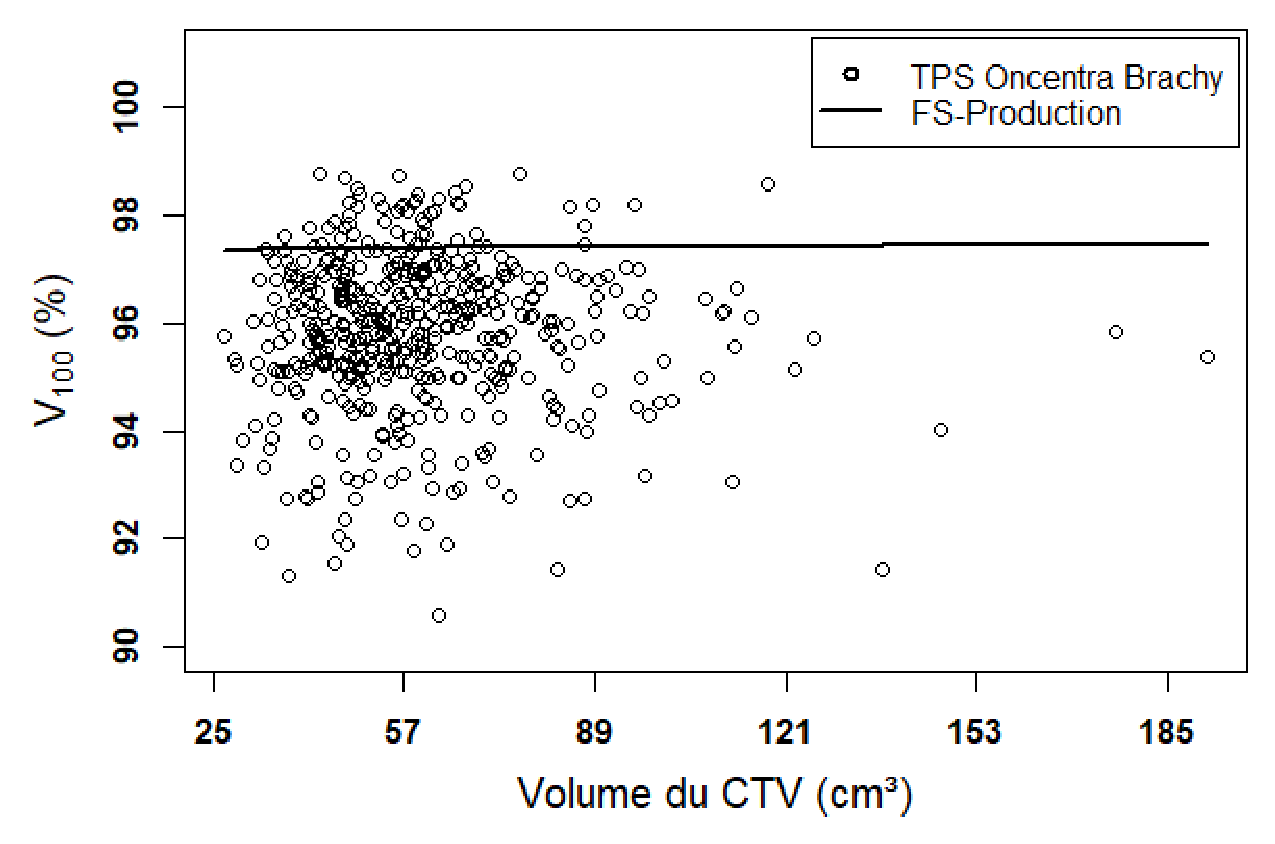
\includegraphics[width=7.2cm,height=5.2cm]{FSV100-CTV}\label{fig:FSV100-CTV}}
  \hspace{0.5cm}
  \subfloat{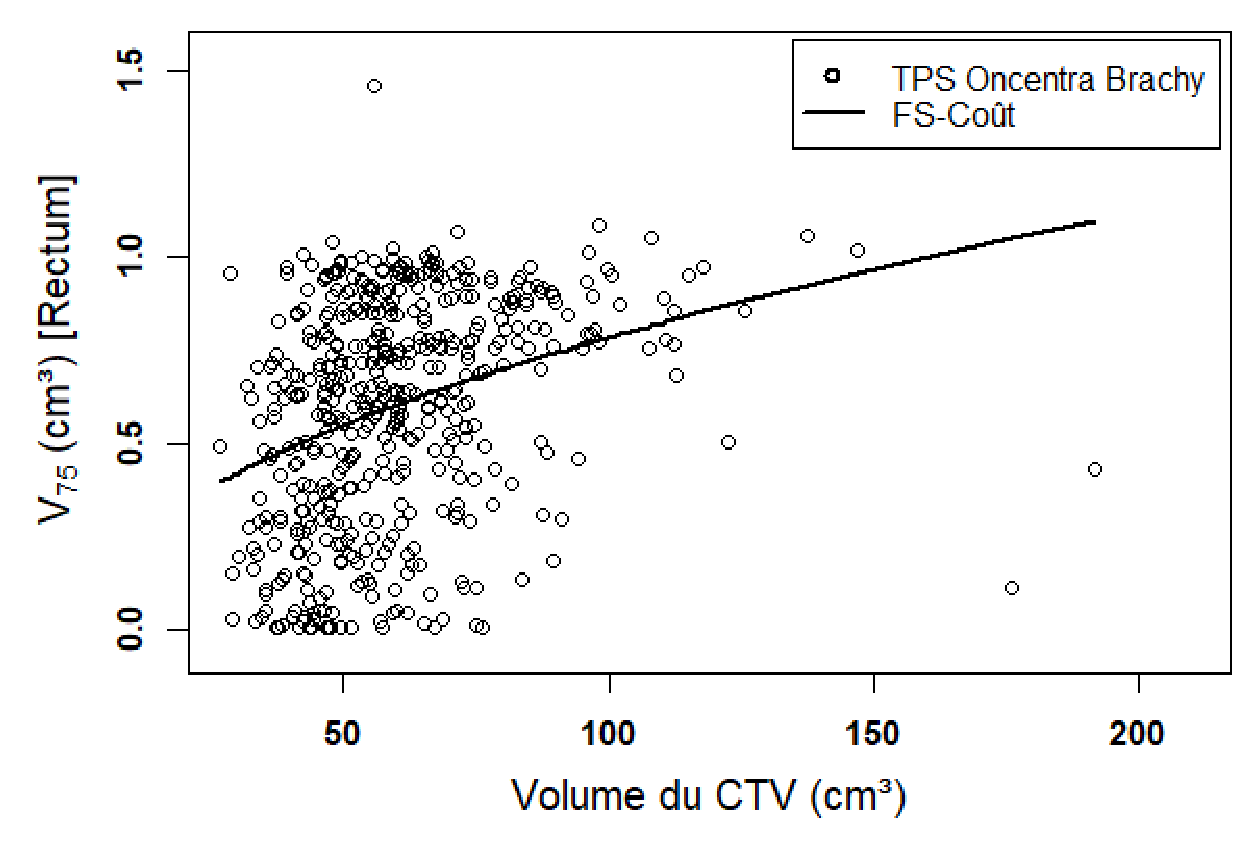
\includegraphics[width=7.2cm,height=5.2cm]{FSV75R-CTV}\label{fig:FSV75R-CTV}}
  \hspace{0.5cm}
  \subfloat{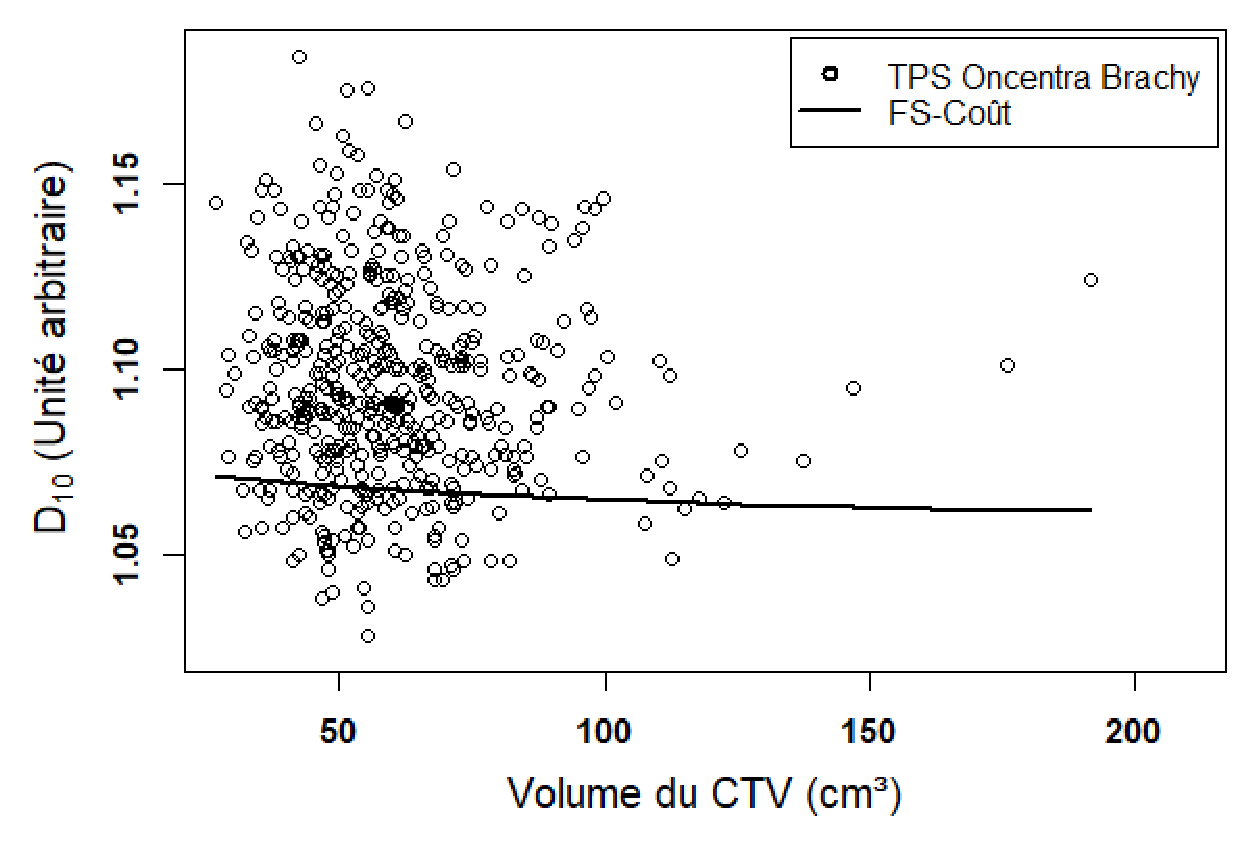
\includegraphics[width=7.2cm,height=5.2cm]{FSD10U-CTV}\label{fig:FSD10U-CTV}}
  \hspace{0.5cm}
  \subfloat{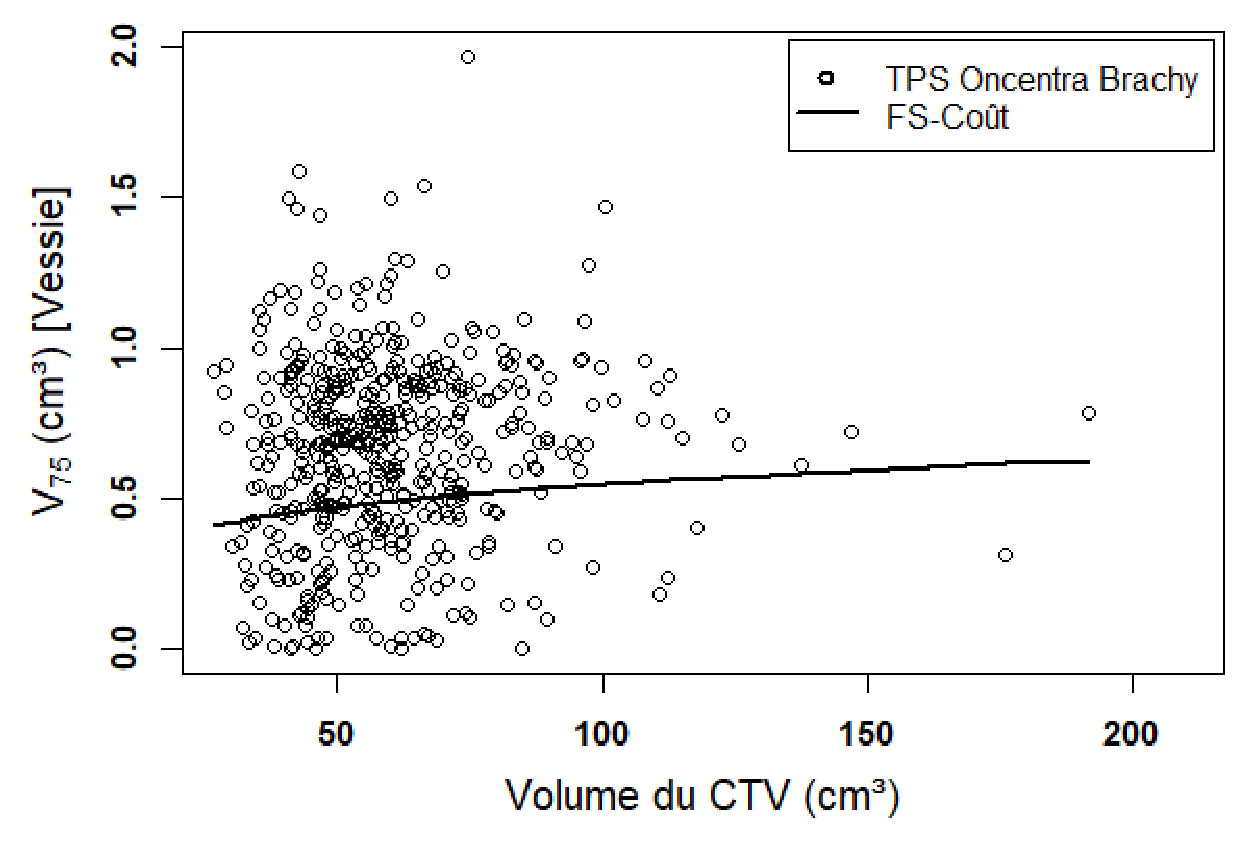
\includegraphics[width=7.2cm,height=5.2cm]{FSV75V-CTV}\label{fig:FSV75V-CTV}}
\caption{\label{ModeleFS-VolCTV} Modèles FS optimisés avec le volume du CTV pour chaque paramètre dosimétrique d'intérêt.}
\end{figure}
%
\begin{figure}[ht!]
  \centering
  \subfloat{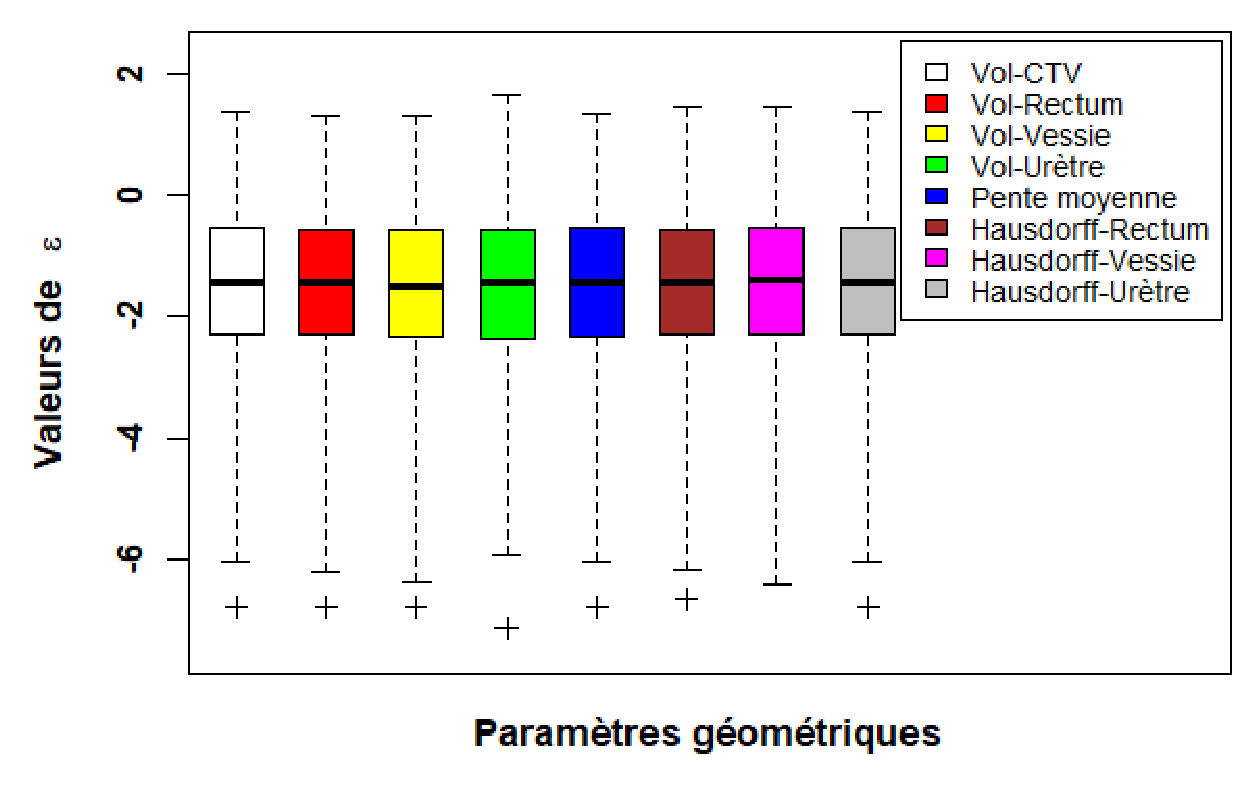
\includegraphics[width=7.2cm,height=5.2cm]{BoxplotCTV}\label{fig:BoxplotCTV}}
  \hspace{0.5cm}
  \subfloat{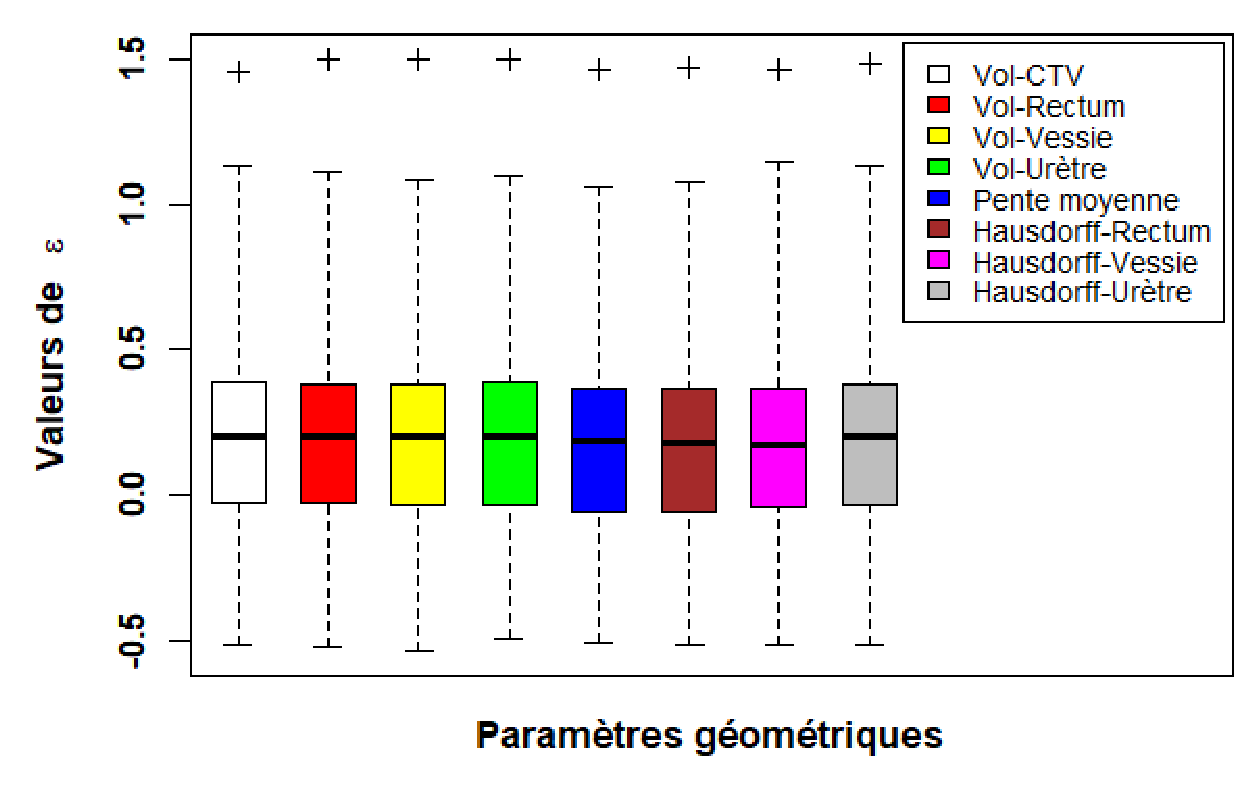
\includegraphics[width=7.2cm,height=5.2cm]{BoxplotV}\label{fig:BoxplotV}}
\caption{\label{ModeleFS-Boxplot} Distribution de $\epsilon$ pour la couverture du CTV (V$_{100}$) et l'indice dosimétrique V$_{75}$ (vessie) en fonction de chaque paramètre géométrique.}
\end{figure}
%
Les valeurs négatives de $\epsilon$ dans la figure \ref{ModeleFS-Boxplot} représentent les plans non optimaux situés en dessous de la FS de production (V$_{100}$), tandis que les valeurs positives de la même variable représentent les plans non optimaux qui sont localisés au-dessus des FS de coût (V$_{75}$, D$_{10}$).
%
\subsection{Modèle de FS complet} \label{subsec:Comb.Lineaire}
\subsubsection{Combinaison linaire des paramètres géométriques}
La construction du modèle global s’est faite en combinant tous les paramètres géométriques selon l’équation \ref{eqn:Chp2Cobb2}.  L’ajout d’un paramètre au modèle fait évoluer la vraisemblance et le test de ratio de vraisemblance donnée par l’équation \ref{eqn:P-value} a été utilisé pour statuer si la variation observée de la vraisemblance suite à l’ajout d’un nouveau paramètre géométrique est statistiquement significative à un seuil de 5\%. La valeur p (p-value) ainsi calculée a permis de déterminer si le modèle à $n$ paramètres est amélioré par rapport à celui de $n-1$ paramètres.
%
\begin{equation}\label{eqn:P-value}
LRT = -2ln\left[\frac{L_{s\left(\theta\right)}}{L_{g}\left(\theta\right)}\right]
\end{equation}
%
$L_{s\left(\theta\right)}$ et $L_{s\left(\theta\right)}$ sont respectivement la valeur de la vraisemblance pour le modèle simple (s, $n-1$ paramètres) et le modèle généralisé (g, $n$ paramètres). La distribution de probabilité du LRT (likelihood ratio test) \nomenclature{LRT}{Likelihood Ratio Test} est gouvernée par une loi du $\chi^{2}$ dont le nombre de degrés de liberté correspond à la différence entre le nombre de paramètres géométriques des deux modèles. La p-value exprimant le risque limite pour lequel on passe de l'hypothèse H$_{0}$ acceptée (le paramète ajouté améliore le modèle) à H$_{0}$ refusée, peut ainsi être calculée avec la fonction de répartition de la loi du $\chi^{2}$ \cite{P-value1,p-value2}. Les tableaux (\ref{ResumeparaFSV100} - \ref{ResumeparaFSD10}) ci-dessous résument les résultats obtenus pour ($\sigma_{u}, \sigma_{v}$), la p-value et $\mathcal{L}$ pour les trois FS (V$_{100}$, V$_{75}$ (vessie) et D$_{10}$ ). La p-value a été calculée en comparant la vraisemblance du modèle à $n$ paramètre par rapport à celui à $n-1$ paramètres (équation \ref{eqn:P-value}). 
%
\begin {table}[ht!]
\captionsetup{singlelinecheck=off, skip=4pt, width =\dimexpr \textwidth-2.5cm\relax}%
 \centering
\caption{Évolution de ($\sigma_{u}, \sigma_{v}$), la p-value et $\mathcal{L}$ en fonction du nombre de paramètres géométriques pour la couverture du CTV. Le modèle de base est constitué du volume du CTV comme paramètre géométrique.}
\label{ResumeparaFSV100}
\vspace{0.2cm}
\renewcommand{\arraystretch}{1.4}
\begin{tabular}{clrrrrrrrrrrr}
\toprule[1.3pt]
\hline
\multicolumn{1}{l} \textbf{Nombre de paramètres} & {} & \multicolumn{5}{c} \textbf{Paramètres du modèle} \\
\cline{3-10}
\multicolumn{1}{c} {géométriques \color{white} es} & {} & $\sigma_{u}$ & {} & $\sigma_{v}$ & {} & p-value & {} & $\mathcal{L}$  \\
\hline
\textbf{Modèle de base} & {} & 1,9887 & {} & 0,8252 & {} & - & {} & 874,302 &  \\
\vspace{0.1cm}
%
\textbf{2} & {} & 1,9875 &  {} & 0,8200 & {} & \textbf{0,0902} & {} & 872,867  \\
% 
\textbf{3} & {} & 1,9970 &  {} & 0,8006 & {} & 0,0159 & {} & 869,962   \\
%
\textbf{4} & {} & 1,9713 &  {} & 0,7787 & {} & 0.0 & {} & 860,949  \\
%
\textbf{5} & {} & 1,9700 &  {} & 0,7765 & {} & \textbf{0,2382} & {} & 860,253  \\
%
\textbf{6} & {} & 1,9592 &  {} & 0,7822 & {} & \textbf{ {\color{red} 0.3452}} & {} & 859,807  \\
%
\textbf{7} & {} & 1,9423 &  {} & 0,7692 & {} & 0,0007 & {} & 854,062  \\
%
\textbf{8} & {} & 1,9504 &  {} & 0,7551 & {} & 0,0492 & {} & 852,129  \\
\bottomrule[1.3pt]
\end{tabular}
\end{table}
%
Les autres paramètres géométriques sont ajoutés au modèle de base dans cet ordre: Vol-rectum, Vol-vessie, Vol-urètre, P-moyenne et Hausdorff CTV-(R, V, U). Vol-x désigne le volume de la structure $x$, P-moyenne est la pente moyenne des cathéter dans la prostate et Hausdorff CTV-(R, V, U) la distance de Hausdorff entre le CTV et le rectum (R), la vessie (V), l'urètre (U).
%
\begin {table}[ht!]
\captionsetup{singlelinecheck=off, skip=4pt, width =\dimexpr \textwidth-3cm\relax}%
 \centering
\caption{Évolution de ($\sigma_{u}, \sigma_{v}$), la p-value et $\mathcal{L}$ en fonction du nombre de paramètres géométriques pour le modèle V$_{75}$ (vessie). Le modèle de base est constitué du volume du CTV comme paramètre géométrique.}
\label{ResumeparaFSV75V}
\vspace{0.2cm}
\renewcommand{\arraystretch}{1.4}
\begin{tabular}{clrrrrrrrrrrr}
\toprule[1.3pt]
\hline
\multicolumn{1}{l} \textbf{Nombre de paramètres} & {} & \multicolumn{5}{c} \textbf{Paramètres du modèle} \\
\cline{3-9}
\multicolumn{1}{c} {géométriques \color{white} es} & {} & $\sigma_{u}$ & {} & $\sigma_{v}$ & {} & p-value & {} & $\mathcal{L}$  \\
\hline
\textbf{Modèle de base} & {} & 0,2176 & {} & 0,2810 & {} & - & {} & 122,593 \\
\vspace{0.1cm}
%
\textbf{2} & {} & 0,2279 &  {} & 0,2764 & {} & 0,0026 & {} & 120,106  \\
% 
\textbf{3} & {} & 0,2316 &  {} & 0,2743 & {} & \textbf{0,0959} & {} & 118,719   \\
%
\textbf{4} & {} & 0,2898  &  {} & 0,2504 & {} & 0,0004 & {} & 112,422  \\
%
\textbf{5} & {} & 0,2533 &  {} & 0,2624 & {} & \textbf{0,1752} & {} & 111,504  \\
%
\textbf{6} & {} & 0,2562 &  {} & 0,2610 & {} & \textbf{{\color{red} 0,6517}} & {} & 111,402  \\
%
\textbf{7} & {} & 0,3094 &  {} & 0,2396 & {} & 0,0062 & {} & 107,655  \\
%
\textbf{8} & {} & 0,2783 &  {} & 0,2466 & {} & 0,0520 & {} & 105,767  \\
\bottomrule[1.3pt]
\end{tabular}
\end{table}
%
\begin {table}[ht!]
\captionsetup{singlelinecheck=off, skip=4pt, width =\dimexpr \textwidth-2.8cm\relax}%
 \centering
\caption{Évolution de ($\sigma_{u}, \sigma_{v}$), la p-value et $\mathcal{L}$ en fonction du nombre de paramètres géométriques pour le modèle D$_{10}$. Le modèle de base est constitué du volume du CTV comme paramètre géométrique.}
\label{ResumeparaFSD10}
\vspace{0.2cm}
\renewcommand{\arraystretch}{1.4}
\begin{tabular}{clrrrrrrrrrrr}
\toprule[1.3pt]
\hline
\multicolumn{1}{l} \textbf{Nombre de paramètres} & {} & \multicolumn{5}{c} \textbf{Paramètres du modèle} \\
\cline{3-9}
\multicolumn{1}{c} {géométriques \color{white} es} & {} & $\sigma_{u}$ & {} & $\sigma_{v}$ & {} & p-value & {} & $\mathcal{L}$  \\
\hline
\textbf{Modèle de base} & {} & 0,0358 & {} & 0,0177 & {} & - & {} & -1077,419 \\
\vspace{0.1cm}
%
\textbf{2} & {} & 0,0356 &  {} & 0,0177 & {} & \textbf{0.1282} & {} & -1078,577  \\
% 
\textbf{3} & {} & 0,0357 &  {} & 0,0177 & {} & \textbf{\color{red} 0,8212} & {} & -1078,602   \\
%
\textbf{4} & {} & 0,0356 &  {} & 0,0176 & {} & \textbf{0,0574} & {} & -1080,407  \\
%
\textbf{5} & {} & 0,0356 &  {} & 0,0176 & {} & \textbf{\color{red} 0,7745} & {} & -1080,448  \\
%
\textbf{6} & {} & 0,0359 &  {} & 0,0173 & {} & \textbf{0,1177} & {} & -1081,672  \\
%
\textbf{7} & {} & 0,0344 &  {} & 0,0179 & {} & 0,0131 & {} & -1084,750  \\
%
\textbf{8} & {} & 0,0340 &  {} & 0,0182 & {} & \textbf{0.3360} & {} & -1085,213  \\
\bottomrule[1.3pt]
\end{tabular}
\end{table}
%
Les paramètres géométriques pour lesquels les p-value résumés dans les tableaux (\ref{ResumeparaFSV100} - \ref{ResumeparaFSD10}) ont une valeur assez différente de la valeur critique de 5\% généralement utilisée dans la littérature ont été supprimées du modèle global; Il s’agit des valeurs mises en évidence en rouge. Les valeurs en gras dans les mêmes tableaux quant à eux, ont été conservées du fait qu’ils sont relativement proches de la valeur critique; le choix de les conserver reste cependant suggestif.\\
Bien que le modèle V$_{75}$ associé au rectum ne présente aucune efficience technique ($\sigma_{u} = 0$), la signifiance statistique de l’ajout de paramètres géométriques supplémentaires au modèle de base a été évaluée quantitativement par la même approche que celle présentée ci-dessus pour les modèles V$_{100}$, V$_{75}$ vessie et D$_{10}$; les résultats sont résumés dans le tableau \ref{ResumeparaFSV75R}. Ces résultats montrent que seuls deux paramètres géométriques (Vol-rectum, Vol-Vessie) semblent ne pas contribuer de façon significative à l’amélioration du modèle, mais tous les paramètres géométriques ont été conservés dans le modèle global, du fait des valeurs de $\sigma_{u} \approx 0$ et $\sigma_{v}$ qui sont relativement constantes quel que soit la p-value. D’autre part, le modèle ne pouvant être utilisé sur le plan prédictif, il n’y a aucun enjeu sur le choix de conserver ou de supprimer les paramètres géométriques ayant une p-value largement supérieure à la valeur critique de 5\%.
%
\begin {table}[ht!]
\captionsetup{singlelinecheck=off, skip=4pt, width =\dimexpr \textwidth-3cm\relax}%
\centering
\caption{Évolution de ($\sigma_{u}, \sigma_{v}$), la p-value et $\mathcal{L}$ en fonction du nombre de paramètres géométriques pour le modèle V$_{75}$ (rectum). Le modèle de bas est constitué du volume du CTV comme paramètre géométrique.}
\label{ResumeparaFSV75R}
\vspace{0.2cm}
\renewcommand{\arraystretch}{1.4}
\begin{tabular}{clrrrrrrrrrrr}
\toprule[1.3pt]
\hline
\multicolumn{1}{l} \textbf{Nombre de paramètres} & {} & \multicolumn{5}{c} \textbf{Paramètres du modèle} \\
\cline{3-9}
\multicolumn{1}{c} {géométriques \color{white} es} & {} & $\sigma_{u}$ & {} & $\sigma_{v}$ & {} & p-value & {} & $\mathcal{L}$  \\
\hline
\textbf{Modèle de base} & {} & 0,0 & {} & 0,2845 & {} & - & {} & 80,165 \\
\vspace{0.1cm}
%
\textbf{2} & {} & 0,0 &  {} & 0,2845 & {} & \textbf{0,9278} & {} & 80,161  \\
% 
\textbf{3} & {} & 0,0 &  {} & 0,2845 & {} & \textbf{0,8215} & {} & 80,135  \\
%
\textbf{4} & {} & 0,0140 &  {} & 0,2824 & {} & 0,0004 & {} & 73,898  \\
%
\textbf{5} & {} & 0,0 &  {} & 0,2799 & {} & \textbf{0,0658} & {} & 72,206  \\
%
\textbf{6} & {} & 0,0193 &  {} & 0,2795 & {} & \textbf{0,2701} & {} & 71,598  \\
%
\textbf{7} & {} & 0,0 &  {} & 0,2744 & {} & 0.0 & {} & 61,861  \\
%
\textbf{8} & {} & 0,0 &  {} & 0,2712 {} & {} & 0,0011 & {} & 56.510 \\
\bottomrule[1.3pt]
\end{tabular}
\end{table}
%
Les valeurs de $\sigma_{u}$ assez élevées du tableau \ref{ResumeparaFSV100} par rapport au bruit aléatoire représenté par $\sigma_{v}$ montrent que, pour l'échantillon considéré, la couverture du CTV est améliorable pour un grand nombre de plans ayant un profil de paramètres géométriques semblables ou identiques, ceci témoigne la signature de la variabilité de la qualité des plans due au jugement et l’expérience du planificateur. Cette signature est moins prononcée pour le modèle de V$_{75}$ (vessie) pour lequel le bruit aléatoire et l’efficience technique sont du même ordre de grandeur ( tableau \ref{ResumeparaFSV75V}). Les résultats concernant le modèle D$_{10}$ (tableau \ref{ResumeparaFSD10}) montrent qu’il y a très peu de marge de manœuvre pour améliorer la dose à cet OAR ($\sigma_{u}$ très faible) à cause sa position dans la prostate. Pour le modèle V$_{75}$ (rectum), certains paramètres géométriques, en l’occurrence : le volume du rectum, le volume de l’urètre et la distance de Hausdorff CTV-Rectum, lorsque pris individuellement tel que présenté dans la figure \ref{ModeleRegres} pour la couverture du CTV, présentent une efficience technique non nulle; bien que celle-ci reste faible comparativement à celle obtenue pour modèle D$_{10}$ de l'urètre (ordre de grandeur 10$^{-2}$ - 10$^{-4}$). Cependant, cette efficience technique s’estompe dès lors que tous les paramètres géométriques sont pris en compte dans une combinaison linéaire pour la construction du modèle global. Ceci témoigne bien l’importance de la prise en compte de tous les paramètres géométriques qui influencent la dose dans cet OAR, en d’autres termes, le caractère prédictif des modèles peut être sous-estimé ou surestimé si les paramètres géométriques contenus dans le modèle ne sont pas assez représentatifs du profil géométrique réel de chaque plan.
%
\subsubsection{Modèles complets}
Chaque modèle complet a pour argument (intrants), la combinaison linéaire des paramètres géométriques jugés statistiquement significatifs sur la base de l'analyse présentée dans la sous-section \ref{subsec:Comb.Lineaire}, et le tableau \ref{GWeight} résume les valeurs des poids des paramètres géométriques $\beta{i}$ de l'équation \ref{eqn:Chp2Cobb2}.
%
\begin {table}[ht!]
\captionsetup{singlelinecheck=off, skip=4pt, width =\dimexpr \textwidth-6.3cm\relax}%
\centering
\caption{Valeurs numériques des paramètres de l'équation \eqref{eqn:Chp2Cobb2} pour les différents modèles, suivies de la statistique de $\epsilon$.}
\label{FrontierNumericalValues} 
\vspace{0.1cm}
\renewcommand{\arraystretch}{1.4}
    \begin{tabular}{crrrrrrrrrrrr}
	\toprule[1.3pt]
	\hline
        Modèles optimisés               &  c     & $\alpha$  & E$(\epsilon)$ & SD \\ 
        \hline
        V$_{100}$ (\%)       & 99,219 & -0,010 & -1,556 &  1,397  \\ 
		V$_{75}$ (B)   		 & 0,122  &  0,304   &  0,169   &   0,300  \\ 
		V$_{75}$ (R)         & 0,867  &   0,489   &  0,0   &   0,271  \\ 
		D$_{10}$ (U)         & 1,216  & -0,023    &  0,027   &   0,027 \\ 
        \bottomrule[1.3pt]
	\end{tabular} 
\end {table}
%
La densité de probabilité de $\epsilon$, dont la statistique est présentée dans le tableau \ref{FrontierNumericalValues} est illustrée dans la figure \ref{DensiteProba} pour le couverture du CTV (V$_{100}$) et la limitation de la dose à l'urètre (D$_{10}$).
%
%\vspace{-0.445cm}
\begin{figure}[ht!]
  \centering
  \subfloat[(Modèle-Couverture du CTV: V$_{100}$)]{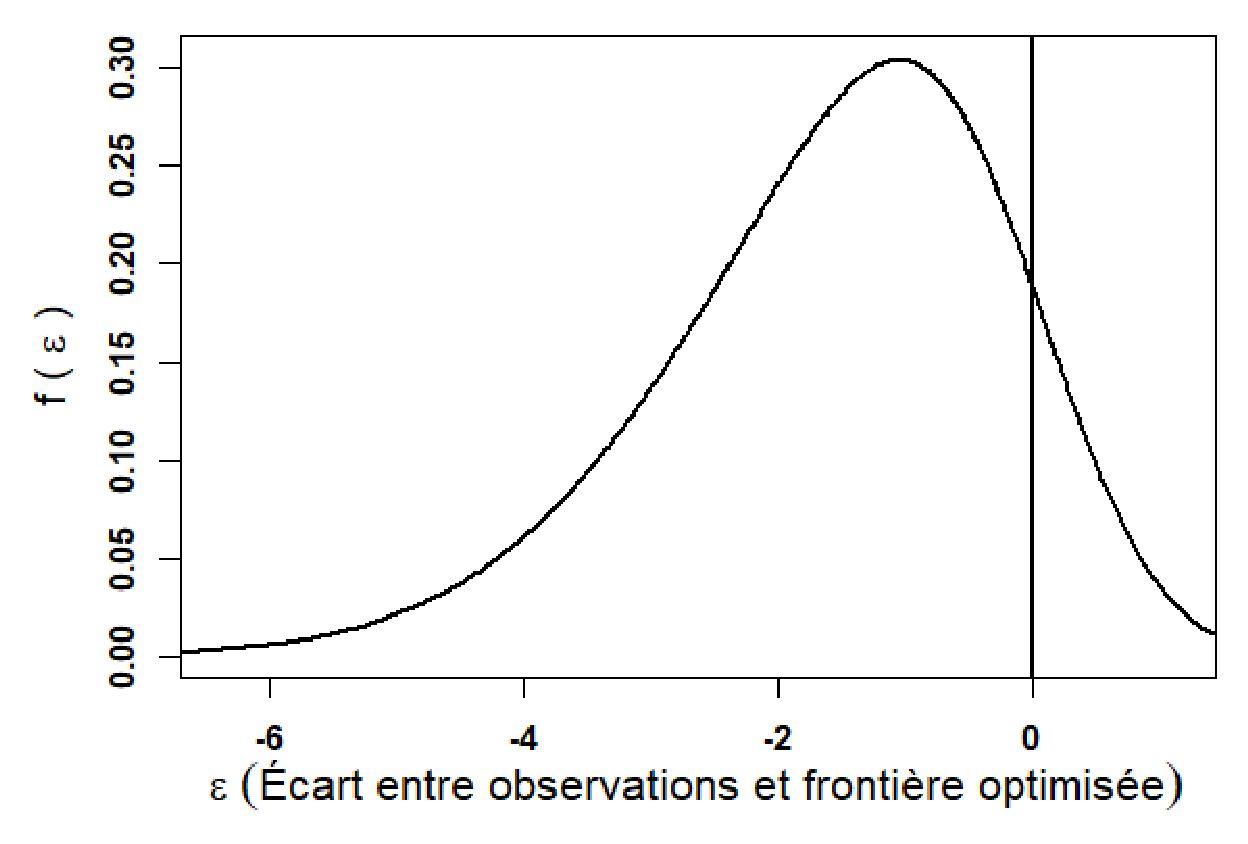
\includegraphics[width=7.2cm,height=5.2cm]{DensiteProba-CTV}\label{fig:DensiteProba-CTV}}
  \hspace{0.5cm}
  \subfloat[(Modèle-Urètre: D$_{10}$)]{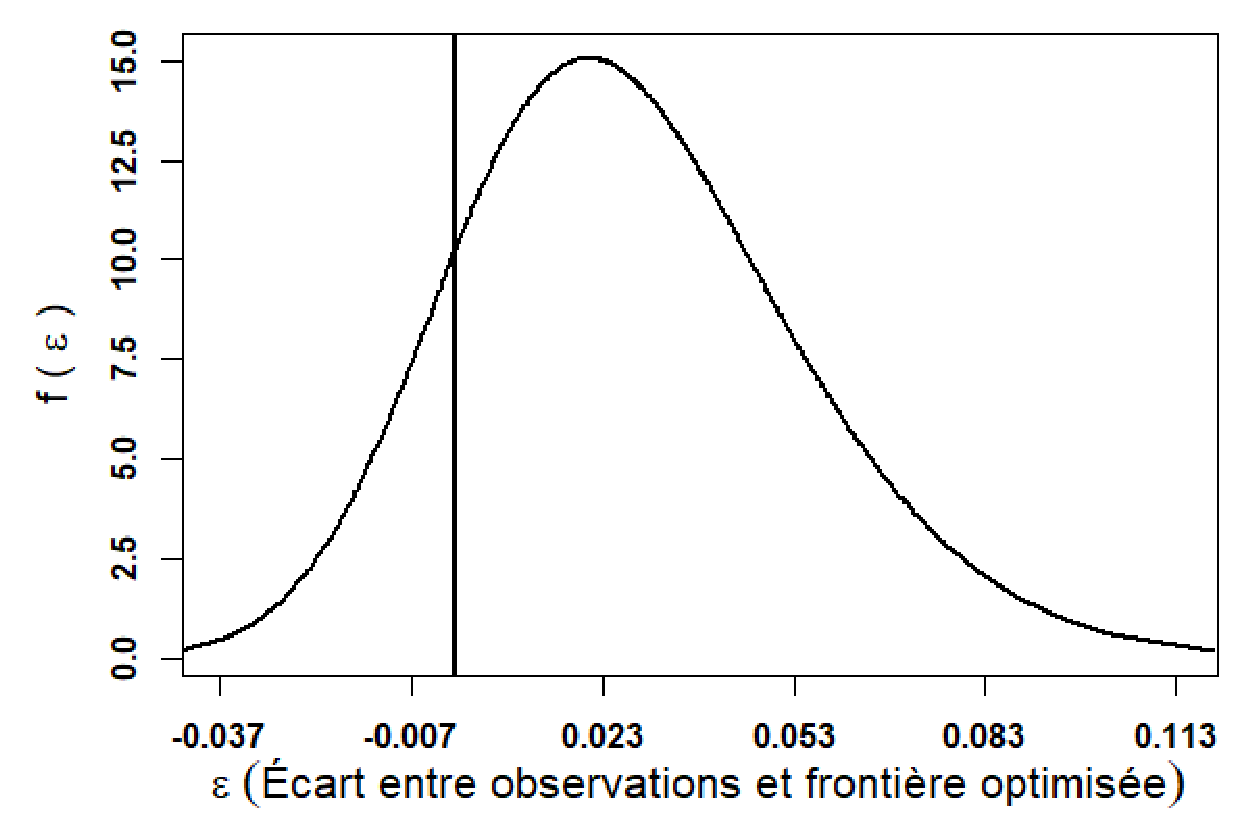
\includegraphics[width=7.2cm,height=5.2cm]{DensiteProba-D10}\label{fig:DensiteProba-D10}}
\caption{\label{DensiteProba} Illustration de la densité de probabilité moyenne relative à la combinaison linéaire des paramètres géométriques pour le modèle correspondant à la couverture du CTV (a) et à la limitation de la dose à l'urètre (b).}
\end{figure}
%
La statistique de $\epsilon$ présentée dans le tableau (\ref{FrontierNumericalValues}) et la distribution de sa densité de probabilité que l'on visualise dans figure \ref{DensiteProba} pour le modèle V$_{100}$ (respectivement D$_{10}$) sont porteurs de quelques informations. En effet, comme attendu, les deux distributions sont tronquées négatives pour V$_{100}$ (respectivement positive pour D$_{10}$) avec les domaines de variabilité compléments différents, à savoir [-6,731; 1.428] (respectivement [-0,045; 0,119]). Ces résultats montrent qu'une amélioration importante ($\epsilon$ assez grand) de la couverture du CTV est possible, comparativement aux résultats de l'urètre. La dispersion élevée autour de la moyenne E ($\epsilon$)  pour le modèle V$_{100}$, comparativement au modèle de l'urètre D$_{10}$ montre la non-uniformité de la qualité des plans pour l'échantillon considéré. Cette dispersion contient une composante liée au jugement et à l'expérience du planificateur, composante qui peut être améliorée pour de nouveaux plans par l'information prédictive contenue dans les modèles. Une analyse similaire peut être menée pour le modèle V$_{75}$ (vessie), mais la statistique de $\epsilon$ présentée dans le tableau \ref{FrontierNumericalValues} montre qu’une amélioration de ce paramètre dosimétrique est possible pour l’échantillon considéré avec une amplitude moindre et peu de variabilité inter-plan en comparaison au cas du modèle associé à la couverture du CTV (V$_{75}$, $\epsilon \in$ [-0,631; 1,493]), mais assez importante en comparaison au modèle associé à la limitation de la dose à l’urètre, D$_{10}$. Les résultats finaux pour les quatre modèles sont illustrés graphiquement dans la figure \ref{ModelGlobalFS} avec les bornes inférieures (Inf.) et supérieures (Sup.) des intervalles de confiances (IC) calculés à 95\% par la méthode Bootstrap avec 4000 Rééchantillonnages. 
%
\begin{sidewaystable}[h!]
\caption{Poids des paramètres géométriques ($\beta{i}$) optimisés pour chaque modèle. Vol-x désigne le volume de la structure $x$ et Hausd-x, la distance de Hausdorff entre le CTV et l'organe $x$; où x désigne le rectum (R), la vessie (V) et l’urètre (U). Pente-moy désigne la pente moyenne des cathéters implantés dans la prostate et SD la déviation standard des deux termes d’erreur, c’est-à-dire, l’efficience technique ($\sigma_{u}$) et le bruit aléatoire ($\sigma_{v}$).  $\beta{i}$ est exprimé en $cm^{-3}$ pour les poids associés aux volumes et en cm$^{-1}$ pour ceux correspondant à la distance de Hausdorff. La pente moyenne (Pente-moy) est une grandeur sans unité.}
\label{GWeight}
\begin{center}
\vspace{-0.5cm}
\renewcommand{\arraystretch}{1.5}
\begin{tabular}{lrrrrrrrrrrrr}
\toprule[1.3pt]
\hline
\multicolumn{1}{l} \textbf{Modèles} & {} & {} & {} & \multicolumn{4}{c} \textbf{Poids des paramètres géométriques ($\beta_{i}$)} & {} & \multicolumn{3}{c} \textbf{SD}\\
\cline{3-10}
\cline{12-13} 
\multicolumn{1}{l} \textbf{optimisés} & {} & Vol-CTV & Vol-Vessie & Vol-Rectum & Vol-Urètre & Pente-moy & Hausd-V & Hausd-R & Hausd-U & {} &  $\sigma_{u}$ & $\sigma_{v}$\\
\hline
\textbf{V$_{100}$ (CTV)} & {} & -0.058 & 0.039 & 0.013 & 3.549 & -4.996 & -0.107 & 0.023 & 0.190 & {} & 1.950 & 0.755 \\
\vspace{0.1cm}
%
\textbf{V$_{75}$ (B)} & {} & 1.756 & 0.953 & 0.654 & -33.488 & -1.731 & -1.730 & - & 0.211 & {} & 0.208 & 0.273 \\
%
\textbf{V$_{75}$ (R)} & {} & 0.007 & 0.002 & 0.001 & -0.048 & 0.441 & -0.008 & -0.002 & 0.015 & {} & 0.000 & 0.271 \\
%
\textbf{D$_{10}$ (U)} & {} & -0.305 & - & -0.950 & 60.091 & - & 3.089 & -0.493 & 2.973 & {} & 0.034 & 0.018 \\
%
\bottomrule[1.3pt]
\end{tabular}
\end{center}
\end{sidewaystable}
%
\clearpage 
CLPG (combinaison linéaire des paramètres géométriques) est le profil de paramètres géométriques caractérisant chaque plan et donné par l'équation,
%
\begin{equation}\label{eqn:ProfilPG}
	\textrm{CLPG} = \sum^{n}_{i=1}\beta_{i}x_{i}
\end{equation}
%
où $n$ est le nombre de paramètres géométriques et $\beta_{i}$ le poids des paramètres géométriques $x_{i}$ résumés dans le tableau \ref{GWeight}. Pour le modèle V$_{100}$ par exemple, CLPG est explicitement donnée par l'équation (\ref{eqn:CLPG}): 
%
\begin{multline}\label{eqn:CLPG}
\textrm{CLPG (Modèle-CTV)} = -0,058.(\textbf{Vol-CTV}) + 0,013.(\textbf{Vol-Rectum}) + 0,039.(\textbf{Vol-Vessie})\\ + 3,549.(\textbf{Vol-Urètre}) - 4,996.(\textbf{Pente-moy}) + 0,023.(\textbf{Hausd-R}) - 0,107.(\textbf{Hausd-V})\\
+ 0,190.(\textbf{Hausd-U})
\end{multline}
%
De façon analogue, le profil de paramètres géométriques (CLPG) pour les autres modèles (V$_{75}$ (vessie, rectum), D$_{10}$) sont facilement déductibles à partir de l'équation (\ref{eqn:ProfilPG}) et des valeurs des poids $\beta_{i}$ résumés dans le tableau \ref{GWeight}. Rappelons que les plans optimaux sont ceux qui sont situés au-dessus de la frontière de production (V$_{100}$) et en dessous de la frontière de coût pour les OARs (V$_{75}$, D$_{10}$).  L’analyse quantitative de la figure \ref {ModelGlobalFS} révèle que la plus grande efficience technique est obtenue pour V$_{75}$ (rectum, $\sigma_{u} = 0$). Ce résultat corrobore avec les informations recueillies auprès des physiciens, selon lesquelles, le rectum est un OAR pour lequel beaucoup d’attention est accordée pour minimiser la dose au cours de la panification, parfois au détriment de la vessie. La plus faible efficience technique est observée pour la couverture du CTV, V$_{100}$. En effet, 83\% des plans sont localisés en dessous de la frontière, avec un écart maximum de 6,4\% par rapport au plan le plus distant de la frontière. En ce qui concerne la vessie (respectivement l’urètre), \textasciitilde 50\% des plans sont situés au-dessus de la frontière de V$_{75}$ avec un écart maximum de 1,28 cm$^{3}$ (respectivement \textasciitilde 72\% des plans au-dessus de la frontière D$_{10}$ avec une différence de dose maximale 1,56 Gy). 
%
\begin{figure}[htp!]
  \centering
  \subfloat{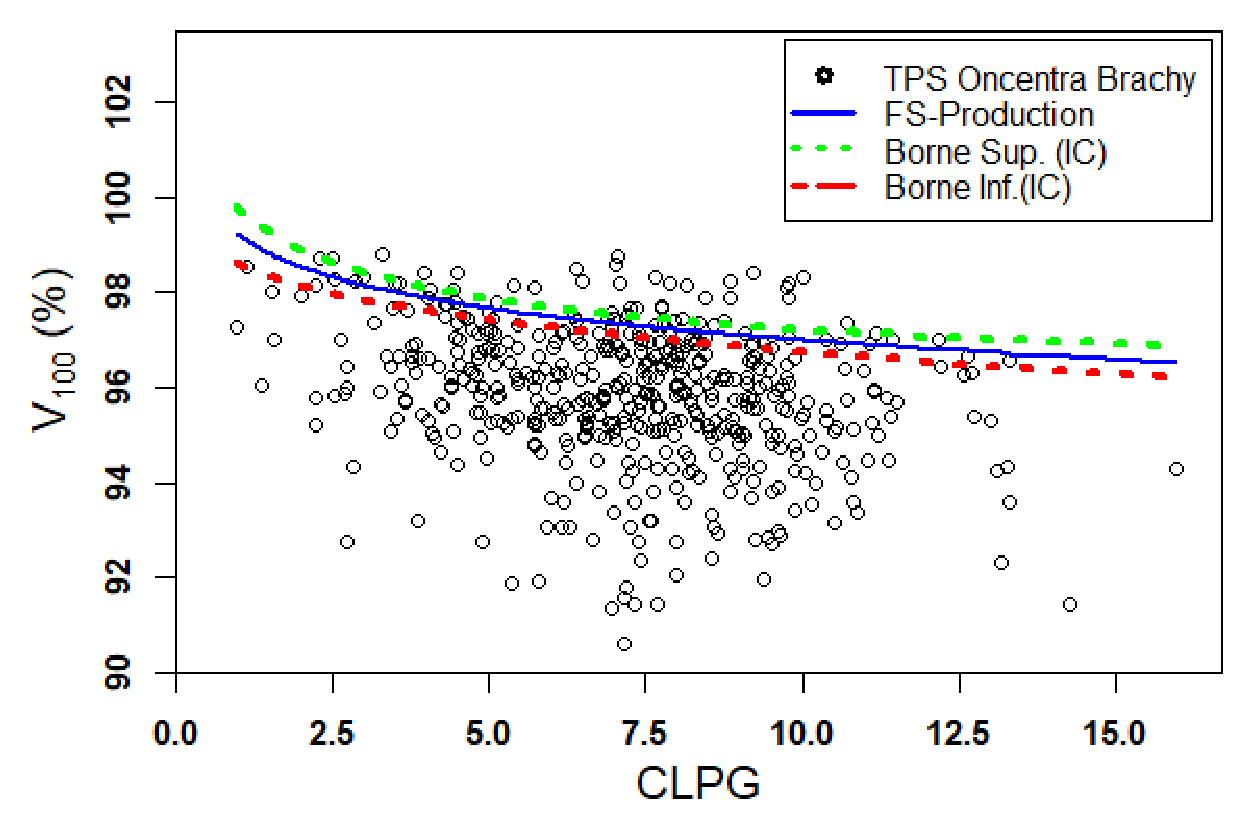
\includegraphics[width=7.2cm,height=5.2cm]{ModeleGlobalV100}\label{fig:ModeleGlobalV100}}
  \hspace{0.5cm}
  \subfloat{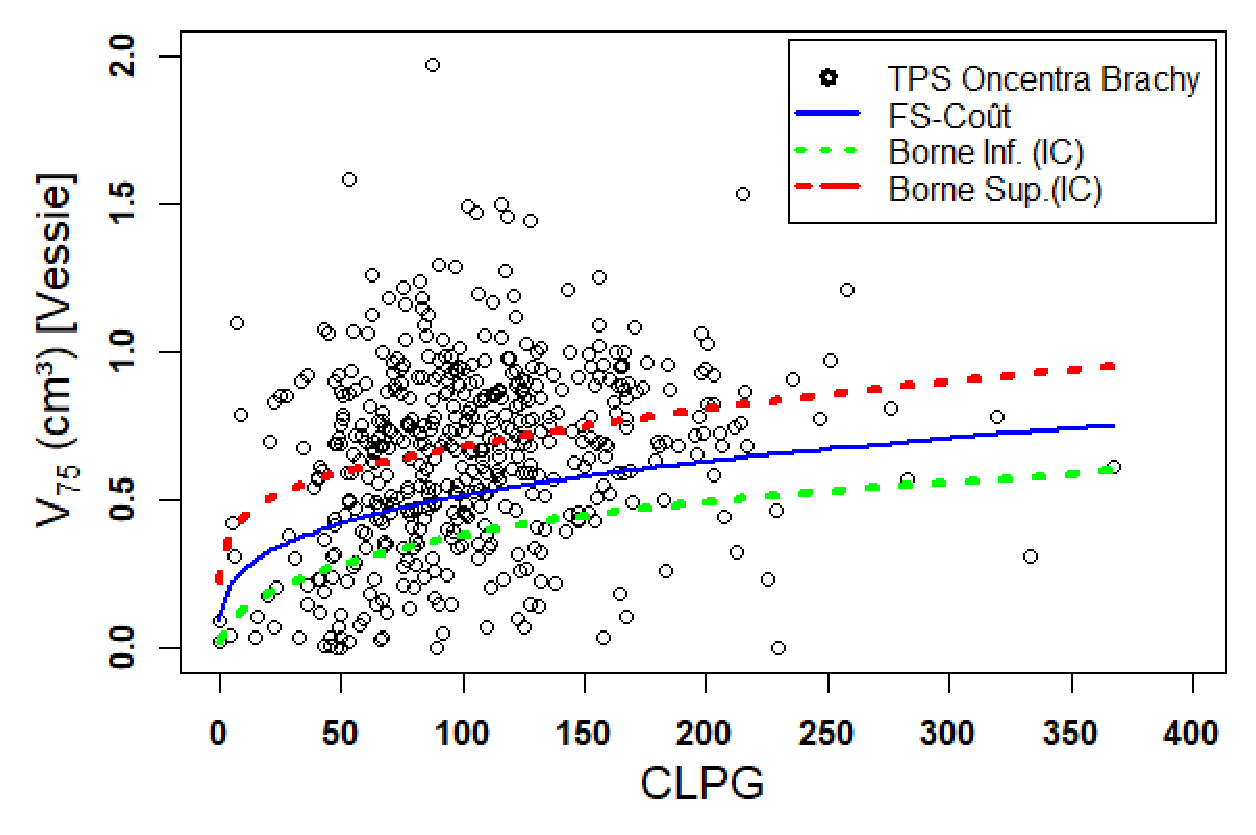
\includegraphics[width=7.2cm,height=5.2cm]{ModeleGlobalV75V}\label{fig:ModeleGlobalV75V}}
  \hspace{0.5cm}
  \subfloat{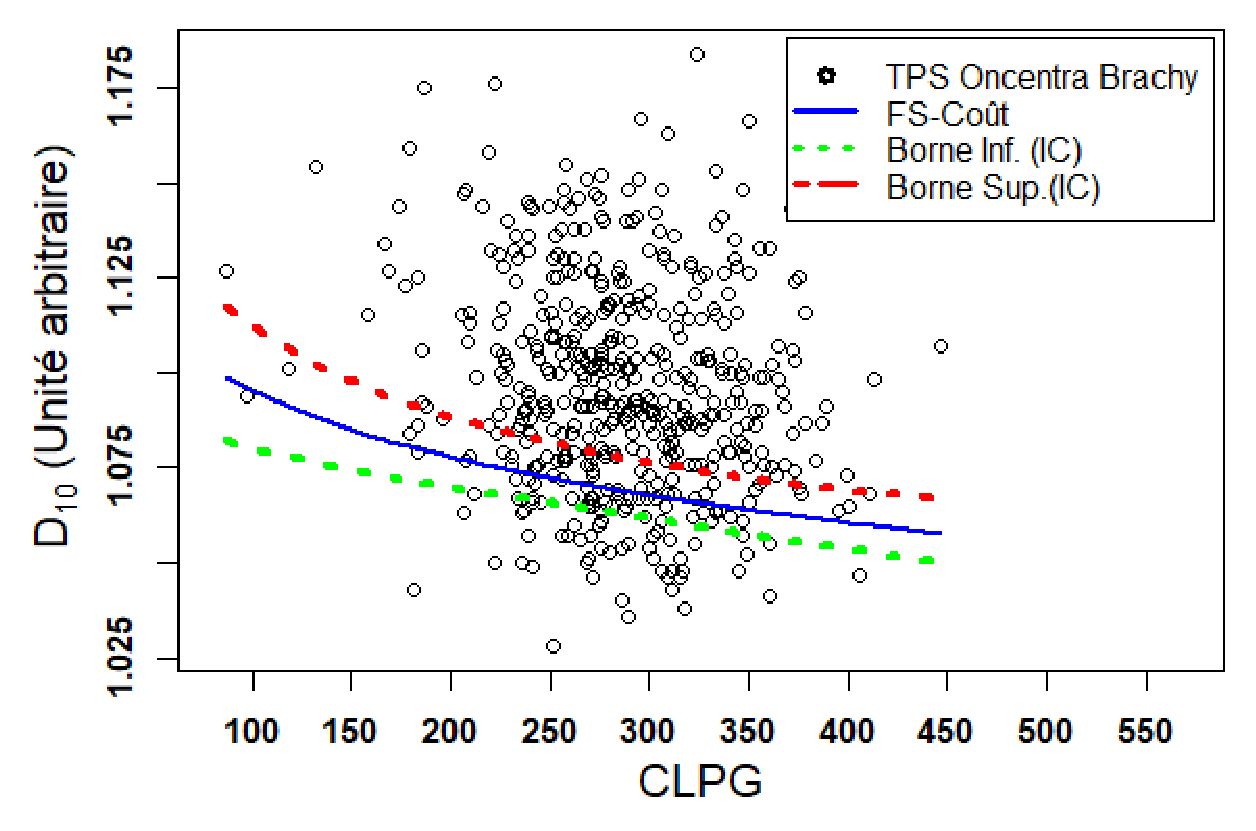
\includegraphics[width=7.2cm,height=5.2cm]{ModeleGlobalD10}\label{fig:ModeleGlobalD10}}
  \hspace{0.5cm}
  \subfloat{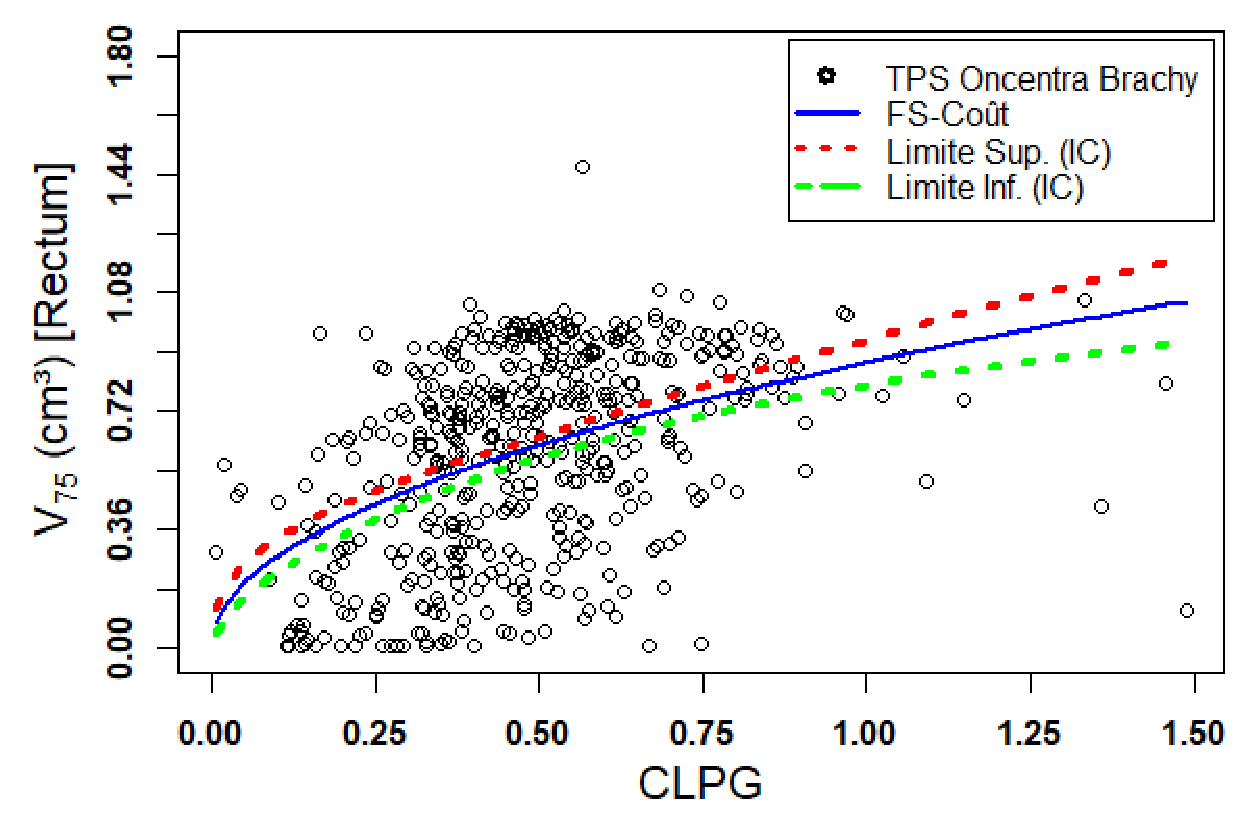
\includegraphics[width=7.2cm,height=5.2cm]{ModeleGlobalV75R}\label{fig:ModeleGlobalV75R}}
\caption{\label{ModelGlobalFS} Modèles de FS complets optimisés pour la couverture du CTV et la limitation de la dose aux OARs (vessie, rectum, urètres). CLPG est la combinaison linéaire des paramètres géométrique qui caractérise chaque plan (voir équation \ref{eqn:CLPG}.}
\end{figure}
%
Le croisement de l'ensemble de l’échantillon pour les trois modèles montre que le nombre de plans qui tombent simultanément dans les régions de confiance est de 3\%, c’est-à-dire, simultanément au-dessus de la frontière V$_{100}$ et en dessous des deux frontières V$_{75}$ (vessie) et D$_{10}$. Ce résultat témoigne le compromis auquel le planificateur est contraint de réaliser, entre la couverture maximale du CTV et la minimisation de la dose aux OARs. Cependant, le planificateur ne dispose d’aucun outil objectif lui permettant de juger sur la pertinence du compromis réalisé. Les présents modèles constituent un outil objectif et robuste pour uniformiser un tel compromis. En effet, un plan pour être considéré comme optimal du point de vue des présents modèles, doit se situer au moins sur chacune des frontières, c’est-à-dire, sur la frontière de V$_{100}$, V$_{75}$ et D$_{10}$; ceci amène à définir deux autres classes de plans, à savoir, les plans fortement optimisés pour la couverture du CTV, mais moins optimisés pour les OARs, inversement. Bien que ces plans restent cliniquement acceptables, le meilleur compromis pourrait correspondre à une situation d’équilibre pour laquelle, on diminue la couverture du CTV, ce qui va favoriser la minimisation de la dose aux OARs, tout en maintenant ledit plan sur ou au voisinage des trois frontières, inversement; 17\% des plans dans l’échantillon peuvent bénéficier d’un tel traitement tout en répondant aux objectifs cliniques.
%
\section{Analyse de l'échantillon test} \label{subsec:Echantest}
Les modèles ont été confrontés à un échantillon test constitué de 100 plans, afin d’évaluer leur capacité à détecter les plans améliorables, plans qui ne font pas partie de l’échantillon ayant servi à la construction des modèles, et par conséquent, mettre en évidence leur pouvoir prédictif. Les résultats quantitatifs détaillés sont présentés dans le chapitre 3 (section \enquote{Testing results}) qui est un projet d’article en voie de soumission. De façon succincte,  il en ressort qu’aucun plan n’a été identifié simultanément dans les régions de confiance des trois modèles. Ces modèles ont également identifié la proportion des plans qui sont améliorables du point de vue de la couverture du CTV et la minimisation de la dose aux OARs, et surtout, la proportion des plans qui peuvent bénéficier d’une augmentation de la couverture du CTV (V$_{100}$) au prix d’une augmentation de la dose aux OARs, mais en maintenant ces derniers en dessous de leurs frontières V$_{75}$ et D$_{10}$. Le pouvoir prédictif des modèles a donc été mis en évidence, ainsi qu’une limitation importante de ces derniers. En effet, le pouvoir prédictif des modèles n’est valable que dans le domaine du profil de paramètres géométriques de l’échantillon sur lequel les modèles sont construits; une proportion de cet échantillon test n’est donc pas incluse dans cette analyse, suite à cette limitation, laquelle peut être améliorée en élargissant la taille de l'échantillon sur lequel les modèles ont été optimisés. 
%
\section{Développements futurs et validation clinique} \label{developementsfuturs}
\subsection{Paramètres géométriques}
Le profil de paramètres géométriques est une donnée importante sur laquelle repose la précision des modèles. Les paramètres géométriques retenus dans ce projet ne sont certainement pas les plus exhaustifs que l’on pourrait imaginer; on pourrait élargir ceux-ci en tenant compte par exemple du gradient d’expansion du volume des OARs (vessie, rectum). En effet, en curiethérapie, les volumes contourés des OARs (vessie, rectum) ne chevauchent pas avec la prostate, mais la mesure de la vitesse avec laquelle un chevauchement aurait lieu (gradient de chevauchement) si une expansion homogène autour de la vessie et le rectum était réalisée pourrait avoir un impact sur la précision des modèles. D’autre part, la distance de Hausdorff prise en compte dans le registre des paramètres géométriques dans cette étude est la distance maximale; on pourrait tester l’impact sur les modèles avec la distance minimale, ou moyenne.
%
\subsection{Ordre des paramètres géométrique}
L’impact de chaque paramètre géométrique du modèle à $n$ paramètres par rapport au modèle à $n-1$ paramètres a été évalué par le biais du calcul de la p-value, mais dans un ordre bien déterminé (voir la section \ref{subsec:Comb.Lineaire}). Une étude sur les différentes permutations possibles en gardant le volume du CTV comme modèle de base, pourrait révéler des informations exploitables dans le sens de l’amélioration des modèles. Cependant, une telle étude va nécessiter une puissance de calcul, car pour le modèle de CTV à 8 paramètres géométriques, cela représente 5040 frontières à optimiser, le modèle de base restant fixe (volume du CTV). 
%
\subsection{\texorpdfstring{Hypothèse de normalité} {Hypothèse de normalité sur u}}
Les résultats présentés dans ce projet reposent sur plusieurs hypothèses dont l’impact sur la précision des modèles mérite d’être évalué. En effet, les modèles sont construits sur l’hypothèse de normalité sur la composante de la variable aléatoire $\epsilon$ qui mesure l’efficience technique, c’est-à-dire, $u$ est distribuée selon une loi normale tronquée positive, $N^{+}(0, \sigma^{2}_{u})$. Bien que cette hypothèse soit largement la plus utilisée dans la littérature, il convient de souligner que d’autres distributions pourraient être testées afin d’évaluer la précision des modèles avec le choix de la distribution de $u$, exemple d’une distribution normale tronquée positive de mode $\mu$ \cite{Stevenson@1980}, ou d'une distribution Gamma \cite{ Greene@1990}. 
%
\subsection{Validation clinique}
Les modèles finaux après un éventuel réajustement au niveau des paramètres géométriques, se doivent d’être validés cliniquement. Cette validation peut se faire de deux façons: (1) replanifier les plans de l’échantillon test qui ont été identifiés comme améliorables (section \ref{subsec:Echantest}), ou (2) confronter les modèles lors de la planification des nouveaux patients. Quel que soit le cas de figure, une analyse doit être faite afin d’évaluer le degré par lequel les valeurs prédites par les modèles sont atteintes ou approchées, et procéder à des ajustements au besoin.
%